\documentclass[pdftex,11pt,a4paper]{report}
\usepackage[portuges]{babel}
\usepackage{amssymb}
\usepackage[utf8]{inputenc}
\usepackage{url}
\usepackage[pdftex]{graphicx}
\usepackage{geometry}
\usepackage{multirow}
\usepackage{verbatim}
\usepackage[usenames,dvipsnames]{color}
\usepackage[a4paper, pdftex, bookmarks, colorlinks,citecolor=darkblue,linkcolor=darkblue,urlcolor=darkblue,filecolor=darkblue]{hyperref}
\usepackage{textcomp} %carregar o euro
\usepackage{rotating} %texto na verticals
\usepackage{fancyhdr}
\usepackage{fancybox}
\usepackage{psboxit}
\usepackage[T1]{fontenc}
\usepackage{fancyvrb}
\usepackage[portuges]{minitoc}
\usepackage{xspace}
\newcommand{\HRule}{\rule{\linewidth}{0.5mm}}
\newcommand\T{\rule{0pt}{2.6ex}}
\newcommand\B{\rule[-1.2ex]{0pt}{0pt}}
\newcommand{\comments}[1]{}
\setlength{\tabcolsep}{15pt}
\frenchspacing

\fancyhead{}
\fancyfoot{}
%% make the odd pages have the section name on the top right
\fancyhead[RO]{\sffamily\bfseries \rightmark}
%% make the even pages have the chapter name on the top left
\fancyhead[LE]{\sffamily\bfseries \leftmark}

%% page nums on the bottom in a nice box
%% even side pages
\fancyfoot[LE]{\psboxit{box 0.8 setgray fill}
{\framebox[10mm][c]{\rule{0cm}{4mm}\color{black}{\bfseries \thepage}}}}
%% odd side pages
\fancyfoot[RO]{\psboxit{box 1 setgray fill}
{\hspace{\textwidth}\psboxit{box 0.8 setgray fill}
{\framebox[10mm][c]{\rule{0cm}{4mm}\color{black}{\bfseries \thepage}}}}}

%% make the bottom line above the page number box
\renewcommand{\footrulewidth}{0.4pt}
\renewcommand{\footruleskip}{0mm}

\pdfpagewidth=\paperwidth
\pdfpageheight=\paperheight

\renewcommand\familydefault{\sfdefault}% usar font sem serifas

% definir acrónimos com itálico
%\renewcommand*{\acf}[1]{\acffont{\textit{\acl{#1}}~\acfsfont{(\acs{#1})}}}

\newtheorem{defin}{Definição}
\geometry{verbose,a4paper,tmargin=30mm,bmargin=30mm,lmargin=20mm,rmargin=20mm}

\pagestyle{fancy}
%\lhead{}
%\rhead{}

%% now redefine the plain style pages (chapter pages, contents pages)
%% to have the same page number stuff on the bottom
\fancypagestyle{plain}{
	\fancyhf{}
	\fancyfoot[RO]{\psboxit{box 1 setgray fill}
	{\hspace{\textwidth}\psboxit{box 0.8 setgray fill}
	{\framebox[10mm][c]{\rule{0cm}{4mm}\color{black}{\bfseries \thepage}}}}}
	\renewcommand{\headrulewidth}{0pt}
	\renewcommand{\footrulewidth}{0.5pt}
}
% %%%%%%%%%%%%%%%%%%%%%%%%%%%%%%%%%%%%%%%%%%%%%%%%%%%%%%%%%%%%%%%%%%
\definecolor{gray_ulisses}{gray}{0.55}
\definecolor{castanho_ulisses}{rgb}{0.71,0.33,0.14}
\definecolor{preto_ulisses}{rgb}{0.41,0.20,0.04}
\definecolor{green_ulises}{rgb}{0.2,0.75,0}

\definecolor{darkblue}{rgb}{0,0.1,0.5}

%% stuff do minitoc %%%%%%%%%%%%%%%%%%%%%%%%%%%%%%%%%%%%%%%
\setcounter{minitocdepth}{2}
\setlength{\mtcindent}{24pt}
\renewcommand{\mtcfont}{\small\rm}
\renewcommand{\mtcSSfont}{\small\bf}
%\newenvironment{mtc}{\secttoc\sectlof\sectlot}{\pagebreak}
%                        ^       ^        ^
%                    conteudos  figuras  tabelas
% \newenvironment{mtc}{\minitoc\minilof\minilot}{\pagebreak}
%%%%%%%%%%%%%%%%%%%%%%%%%%%%%%%%%%%%%%%%%%%%%%%%%%%%%%%%%%%
%\usepackage{hyphenat}
%\hyphenpenalty=10000 %remover hifenização nas mudanças de linha
\renewcommand\familydefault{\sfdefault} %usar font sem serifas

\begin{document}
\begin{titlepage}
\thispagestyle{empty}
{\centering \large
{\large\bf \textbf{Universidade do Minho} \\ Departamento de Informática}\\
\vspace{1cm}
\bf{UCE15}\\
\vspace{2cm}
\vspace{1cm}
{\LARGE \textbf{Delusion}}\\
\vspace{1cm}
{\Large The biggest defense is deception}\\
\vspace{1cm}
\vspace{8.5cm}
}

\flushleft{ \emph{Grupo:\\}
\vspace{0.4cm}
\begin{tabular}{llll}
Mário Ulisses Costa & pg15817 & Luís Ferreira & pg18779 \\
Pedro Faria & pg17684 & Pedro Vieira & pg17803 \\
Rui Gonçalo & pg18378 & Ricardo Alves & pg17904 \\
Leonel Braga & pg17311 & Ricardo Ferreira & pg18375 \\
Renato Neves & pg17229 & João Peixoto & pg19811 \\
Jorge Mendes & pg16490 &  Marco Carneiro & pg17774\\
Eduardo Conceição & pg17211 && 
\end{tabular}
\\
}
\vspace {1.5cm}
\textbf{Braga, \today}\\
\pagebreak
\end{titlepage}

\pagenumbering{roman}
% indices
\dominitoc
\dominilof
\renewcommand{\contentsname}{Índice}
\tableofcontents
\addcontentsline{toc}{chapter}{\contentsname}
\renewcommand{\listfigurename}{Índice de Figuras}
\listoffigures
\addcontentsline{toc}{section}{\listfigurename}
\renewcommand{\listtablename}{Índice de Tabelas}

\newpage
\pagenumbering{arabic}
\addtocounter{mtc}{+1}
\chapter{Informação do Projecto}
\section{Motivação do Projecto}
\subsection{Contexto}
Nos dias que correm, é fundamental para as seguradoras a disponibilização de simuladores de seguro aos seus clientes, o que constitui um excelente modo de publicitar as suas inovações no desenho da fórmula de cálculo do prémio.
A inexistência no mercado de um simulador que agregue múltiplos seguros constituiu uma oportunidade para o desenvolvimento deste projecto, com grande potencial de interesse por parte das seguradoras, visto oferecer-lhes a vantagem de publicitar os seus descontos multi-seguro.
\subsection{Objectivo do Projecto}
O objectivo do projecto é informatizar um sistema na área de seguros, isto é, desde a simulação à contratação e configuração dos seguros. Com esta informatização pretende-se que os utilizadores do sistema consigam realizar o processo com mais facilidade. Também será desenvolvido um simulador multi-produto que junte às simulações unitárias toda a área de atribuição de descontos justificada pela multiplicidade de seguros.

\section{\emph{Stakeholders}}

\subsection{Cliente}
Deloitte (Representante: João Lúcio Borbinha)

\subsection{Comprador}
Companhias de Seguros

\subsection{Outros \emph{Stakeholders}}
Professores (\emph{input} de conhecimento técnico e supervisão do projecto):
\begin{itemize}
\item João Miguel Fernandes
\item Fernando Mário Martins
\item José Alberto Saraiva
\item Olga Maria Pacheco
\end{itemize}
\subsection{Os Utilizadores do Produto}
\begin{description}
\item \textbf{Utilizador 1}
\item Categoria: 

Recém-proprietários de um veículo automóvel
\item Responsabilidades do utilizador: 

Tem a obrigação de criar um seguro após a compra do carro.
\item Nível de conhecimento tecnológico: 

Conhecimentos básicos
\item Outras características importantes:

Idade igual ou superior a 18\\\\
\end{description}
\begin{description}
\item \textbf{Utilizador 2}
\item Categoria: 

Utilizadores descontentes com o seu seguro actual
\item Responsabilidades do utilizador: 

Tem um seguro já criado
\item Nível de conhecimento tecnológico: 

Variado
\item Outras características importantes: 

Vontade de mudança, aberto a sugestões. Idade igual ou superior a 18.\\\\
\end{description}

\subsection{\emph{Personas}}
\begin{description}
\item \textbf{Rui}

51 anos, casado, 2 filhos

Advogado, viaja com frequência

Gosta de futebol e de dançar

A família é o mais importante para ele

\item \textbf{Paula}

25 anos, solteira

Agente de seguros

Organizada e gosta de fazer compras

Gosta de fotografia e viajar

Gosta de novas tecnologias

\end{description}
\pagebreak
\subsection{Prioridade dos Intervenientes}

\begin{figure}[!htb]
     \centering
%     \includegraphics[scale=0.8]{images/piramide}
     \caption{Prioritização dos intervenientes}
\end{figure}

\subsection{Contribuição dos Intervenientes}
O cliente João Borbinha transmitiu ao grupo de trabalho conhecimento sobre o modelo de negócio em causa, e acompanhamento/aconselhamento periódico em relação às dúvidas resultantes do levantamento de requisitos. 

Pelo contacto realizado com um agente de seguros, obtivemos informação relevante sobre o processo da contratação nos seguros Automóvel e Saúde.

\subsection{Suporte e Manutenção}
Para suporte e manutenção estarão destacados os Administradores do sistema, técnicos que se espera terem conhecimento informático médio/alto, suficiente para executar a função com recurso apenas à documentação disponível (independentes dos developers originais).

 %done
\chapter{Restrições do Projecto}
\section{Restrições impostas}
\subsection{Restrições de Solução}

\begin{figure}
	\centering	
	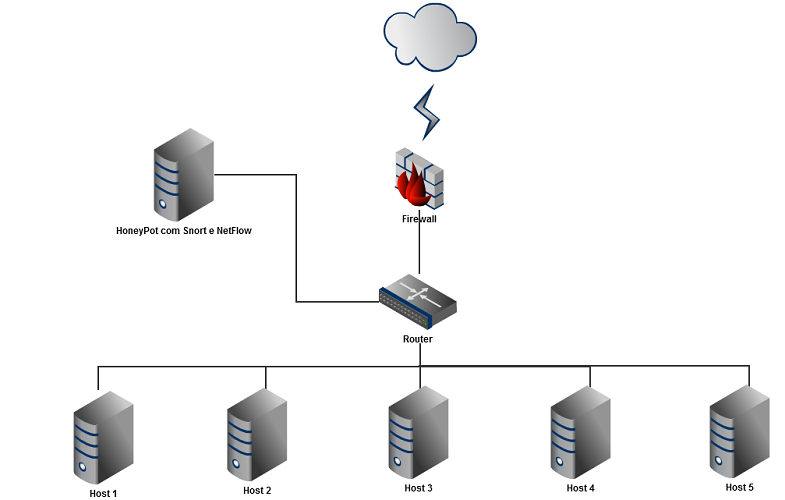
\includegraphics[scale=0.7]{images/topologia1.png}
	\caption{Topologia de Rede 1}
\end{figure}

\begin{figure}
	\centering	
	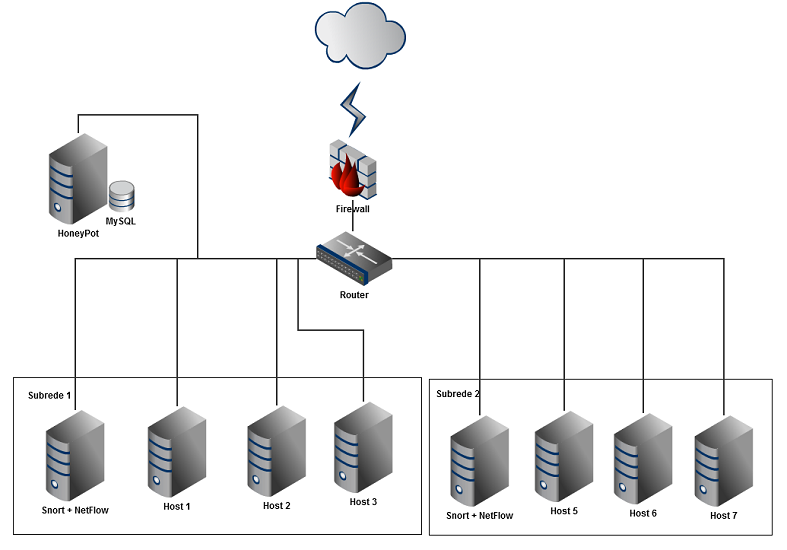
\includegraphics[scale=0.7]{images/topologia3.png}
	\caption{Topologia de Rede 2}
\end{figure}


\subsection{Ambiente de Instalação do Sistema}


Este produto é destinado a ser instalado nos servidores de cada uma das companhias de seguros compradoras. Devido a essa multiplicidade o ambiente tecnológico esperado deve manter-se universal, não contemplando nenhuma especificação particular a um determinado tipo de configuração empresarial.

\subsection{Aplicações Associadas}
Como o produto se destina a uma multiplicidade de empresas, não é possível saber com que software vai ser integrado. Contudo, para facilitar tal integração com outros \emph{softwares} da empresa, será criada uma API documentada no manual de funcionamento para promover a interacção entre este software e outros já existentes.

\subsection{Software Off-the-Shelf}
\begin{description}
    \item [Visual Paradigm for UML 7.1 Community Edition] usado para modelar o sistema de negócio e o sistema informático
    \item [Volere Template] usado como guia para elaborar o documento de requisitos

\end{description}

\subsection{Ambiente de Trabalho}
Os Utilizadores(Registado e Anónimo) do produto irão aceder ao sistema de onde pretenderem, em qualquer dispositivo electrónico que suporte o acesso \emph{web} e a tecnologia Java.

Os Mediadores executarão as suas funções laborais maioritariamente no seu local de trabalho (delegações, call-center), assim como os Colaboradores. No entanto, poderão também executá-las nos mesmos moldes que os Utilizadores anteriormente descritos.

Como este simulador de seguros não recebe nem é afectado por qualquer \emph{input} do ambiente físico exterior, estes ambientes expectáveis não terão influência directa no desenho do sistema.

\subsection{Restrições de Calendário}
\begin{description}
    \item 12 de Novembro de 2011 - Visão do Produto: 
        \begin{itemize}
            \item Análise de mercado
            \item Modelo de negócio, proposta de valor e avaliação da oportunidade
            \item Documento de Requisitos
        \end{itemize}
    \item 14 de Janeiro de 2012 - Documentação Técnica e de Instalação: 
        \begin{itemize}
            \item Produto de software
            \item Manuais de utilização
        \end{itemize}
    \item 11 de Fevereiro de 2012 : Visão Final do Produto:
        \begin{itemize}
            \item Documento de Requisitos
            \item Plano do projecto
            \item Documento do estado do projecto
            \item Documentação técnica e de instalação
            \item Produto de software
            \item Manuais de utilização
        \end{itemize}
    \item 18 de Fevereiro de 2012 : Apresentação Final: 
        \begin{itemize}
            \item Apresentação final
            \item Exposição dos trabalhos
        \end{itemize}
\end{description}

\section{Nomenclatura e Definições}
\subsection{Termos Usados no Projecto}

Ver Anexo ~\ref{appendix:1}.

%Requesitos funcionais
\chapter{Requisitos Funcionais}
\minitoc
\section{Âmbito do projecto}
\subsection{Situação actual}
Actualmente, o mercado de segurança em redes informáticas disponibiliza uma grande variedade de sistemas de segurança, sob vários pontos de vista.
Estes sistemas podem tomar a forma de sistemas de prevenção a ataques a uma rede com serviços, protecção contra ataques, através da
escrita de regras de acesso à rede e ainda análise de ataques.\\
Todos estes serviços/produtos geram informação que é necessário que é lida pelo administrador de rede, afim de compreender o tipo de ataque que houve,
se o sistema de protecção foi eficaz e se não, tentar melhorar o sistema em causa.\\
Muitas vezes estes sistemas geram ficheiros de log muito grandes e practicamente complexos para um humano interpretar e extraír informação.\\
Suprir esta lacuna é o mote para o desenvolvimento deste produto que deverá mostrar através de uma forma clara os ataques que uma rede foi alvo
e ainda os ataques que o honeypot sofreu. Por forma a que o administrador de rede compreenda facilmente e na totalidade o tipo de ataque que a sua rede sofreu.
Com esta informação espera-se que a tarefa de melhorar a segurança de rede seja facilitada ao administrador.

\subsection{Contexto do projecto}
Por forma a dar uma melhor ideia geral da arquitectura do projecto e por forma a mostrar de que forma a compreender
a interacção das várias entidades do sistema (quer sejam humanas ou não) é imperativo que se modele um diagrama de contexto.
Neste diagrama iremos mostrar quais as entidades externas ao sistema informático que vão ter algum relacionamento com este, 
isto é, quais as actividades que o sistema informático vai suportar no negócio em questão. 

\subsection{Diagrama de Contexto}
Para explicar com maior detalhe o sistema de que estamos a falar mostramos na Figura \ref{fig:dcont} o diagrama de contexto.

\begin{figure}[!ht]
\centering
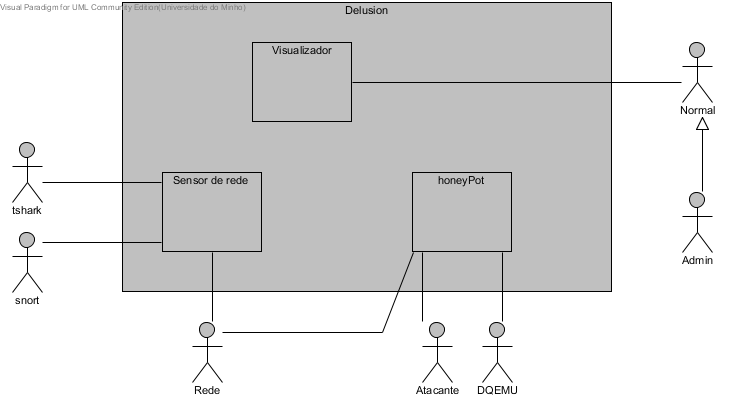
\includegraphics[scale=0.8]{images/DiagramaContexto}
\caption{Diagrama de Contexto}
\label{fig:dcont}
\end{figure}

Como se pode ver nesse diagrama apresentamos os três elementos mais importantes deste projecto, o Visualizador, o Sensor de rede e o Honeypot.
O Visualizador apresenta uma interface web para o utilizador deste sistema, o Sensor de rede usa como entidades externas duas ferramentas para fazer inspecção
ao nível de rede: o tshark e o snort. Ainda temos o componente de Honeypot que usa o DQEMU (a ferramenta que vamos desenvolver), este sistema tem ainda
como actor o atacante, pois este irá ser atraído para este sistema e será gravada toda a sua actividade dentro do Honeypot.\\
Existem dois tipos de utilizadores do Visualizador: O utilizador Admin que tem total controlo sobre o sistema, podendo ler informação sobre os ataques, bem como
criar novos honeypots na rede com determinadas caracteristicas. Temos ainda o utilizador Normal que terá os mesmos privilégios que o Admin, mas apenas num
segmento menor da rede, segmento esse que será o Admin a atribuir.


 %done
\section{Modelos de Domínio}
Se seguida mostramos os vários diagramas referentes à interligação ds várias entidades de domínio.\\
Na Figura \ref{fig:mdgeral} temos uma visão geral (de nível 0) do modelo de domínio deste projecto. Vemos que existem dois tipos de utilizadores (Normal e Admin)
que acedem ao Visualizador. O Visualizador por si só mostra informação sob a forma de esquemas que podem ser gráficos ou tabelas sobre os ataques.\\

Introduzimos aqui também a noção de plugin, que pode ser visto como um conjunto de contractos que todos os sistemas teêm de cumprir se quiserem desenhar
algum esquema no Visualizador. Portanto podemos ver estes sistemas como webservices que comunicam com o Visualizador para desenhar esquemas.\\

Neste caso, definimos que o produto minimo seria o conjunto de dois sensores um ao nível de rede e outro ao nível do sistema operativo (o Honeypot).
Com estes dois sistemas teremos então cumprido o objectivo principal deste projecto - identificar ataques ao nível de rede e de sistema operativo.\\
O sistema de Sensor de rede usa uma Base de dados para registar o tráfego de rede e os alertas lançados pelo snort. Por outro lado o honeypot
detecta os ataques e regista também na Base de dados estes ataques.

\begin{figure}[!ht]
\centering	
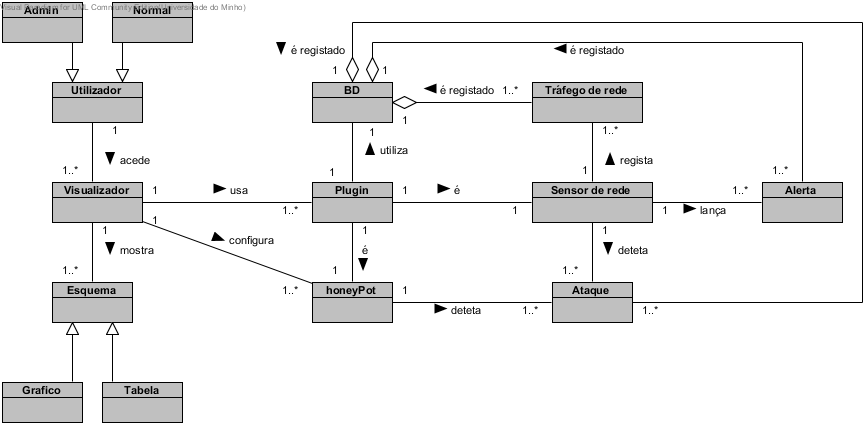
\includegraphics[scale=0.7]{images/ModelosDeDominio/Geral.png}
\caption{Modelo de Domínio Geral}
\label{fig:mdgeral}
\end{figure}

Na Figura \ref{fig:mdhoney} podemos ver o modelo de domínio do Honepot em maior detalhe. É importante referir que este projecto
prevê que o Honeypot esteja a correr numa máquina virtual, porque assim facilita a inspecção. Neste nível de granularidade vemos que existem duas entidades,
uma o sistema operativo Host que é o sistema operativo que corre a máquina virtual e o sistema operativo guest, que é o sistema operativo virtualizado.
O sistema operativo host possui várias instâncias de máquinas virtuais alteradas a que demos o nome de DQEMU, que será um sistema de virtualização
com a capacidade de inspeccionar a actividade do sistema operativo guest. O DQEMU, que supervisiona o guest, quando detectar actividade maliciosa no guest
armazena informação sobre essa actividade na base de dados.\\
De lembrar que o guest possuí propositadamente vulnerabilidades com o intuito de atrair atacantes e assim registar as suas actividades.\\
Este guest pode ter várias personalidades, isto é sistemas operativos reais a correr, entre elas: Linux, Solaris e Windows.

\begin{figure}[!ht]
\centering	
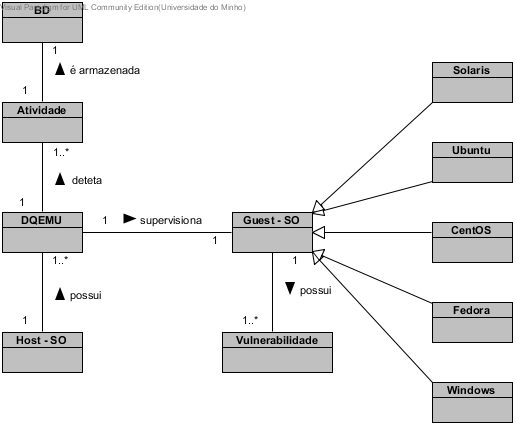
\includegraphics[scale=0.8]{images/ModelosDeDominio/HoneyPot.png}
\caption{Modelo de Domínio HoneyPot}
\label{fig:mdhoney}
\end{figure}

A Figura \ref{fig:mdrede} apresenta o modelo de domínio do sensor de rede, que neste caso será o conjunto de três ferramentas, sendo que uma delas será
construída no ambito deste produto - o Delusion collector daemon. Aqui irá ser necessário utilizar as informações que o tshark e o snort collectam da rede
afim de tirar conslusões sobre a acitivade da rede. Será ainda utilizada uma Base de dados para guardar os alertas do snort e o trágefo de rede, devidamente relacionado
e ainda fazer polling dos alertas do snort.

\begin{figure}[!ht]
\centering	
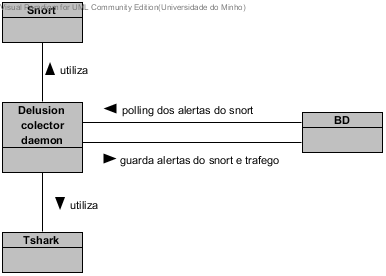
\includegraphics[scale=0.8]{images/ModelosDeDominio/Rede.png}
\caption{Modelo de Domínio Rede}
\label{fig:mdrede}
\end{figure}

A Figura \ref{fig:mdvis} apresenta o modelo de domínio do visualizador onde se pode ver um Filtro que o utilizador usa para restringir a amostragem de
informação (por exemplo pode ser: "mostra-me todos os alertas de ataques das últimas 24 horas"). Este Filtro irá usar a Base de dados para extraír a informação
pretendida e posteriormente esa informação será mostrada em forma de gráfico ou tabela.

\begin{figure}[!ht]
\centering	
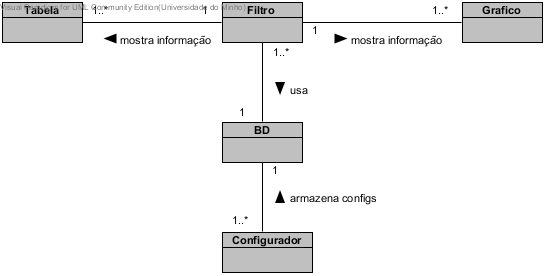
\includegraphics[scale=0.8]{images/ModelosDeDominio/Visualizador.png}
\caption{Modelo de Domínio Visualizador}
\label{fig:mdvis}
\end{figure}
\pagebreak
 %done
\newpage
\section{Modelos de Casos de Uso}
\subsection{Modelo de Casos de Uso de alto nível}
Diagrama geral de Use Cases

\begin{comment}
\begin{figure}[!htb]
	\centering
	\includegraphics[scale=0.85]{images/diagramaGeralDeUseCase}
	\caption {Diagrama geral de \emph{Use Cases} do produto}
\end{figure}
\end{comment}

\subsection{Modelos de Casos de Uso detalhado}
\subsubsection{\textbf{1 - HoneyPot}}
\begin{itemize}
 \item \textbf{Identificar system calls e actualizar BD} -  Tal como apresentado no diagrama abaixo, o QEMU é capaz de identificar system calls
 do guest OS mais seu contexto. Após detectar uma chamada este actualiza a Base de dados com essa informação. 
 \item \textbf{Copiar ficheiros} - O QEMU pode também copiar qualquer ficheiro do guest OS para o Host OS ou para outro ponto remoto.
 \item \textbf{Filmar HoneyPot} - Mais ainda o QEMU é capaz de capturar uma sequência de capturas de ecrã do que se passa no guest, 
 criando assim um ficheiro em formato vídeo para, mais tarde o utilizador poder ver.
 \end{itemize}

\begin{figure}[!ht]
	\centering
	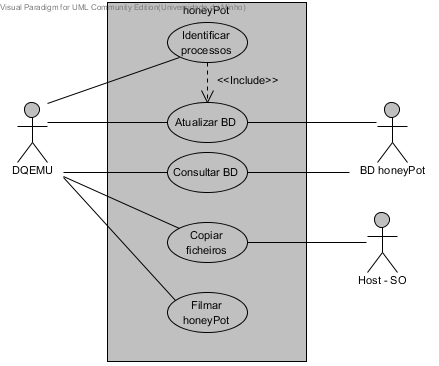
\includegraphics[scale=0.80]{images/ucs/HoneyPot}
	\caption {Diagrama de use case, parte do HoneyPot}
\end{figure}
\pagebreak

\subsubsection{\textbf{2 - Rede}}
\begin{itemize}
 \item \textbf{Captura trâfego} - O Snort e o TShark tem como função capturar todo o tipo de trâfego que passe pela rede. Toda essa informação
 irá convergir para o Delusion Collector Daemon (DCD) que irá registar essa informação na base de dados.
 \item \textbf{Filta trâfego} - O TShark pode adicionalmente filtrar o tráfego que coleta segundo critérios escolhidos pelo utilizador
 \item \textbf{Analisa trâfego} - O Snort irá analisar o tráfego e procurar por padrões de eventos maliciosos, quando encontrar um padrão gera um
 alerta, que será capturado pelo DCD.
 \end{itemize}

\begin{figure}[!ht]
	\centering
	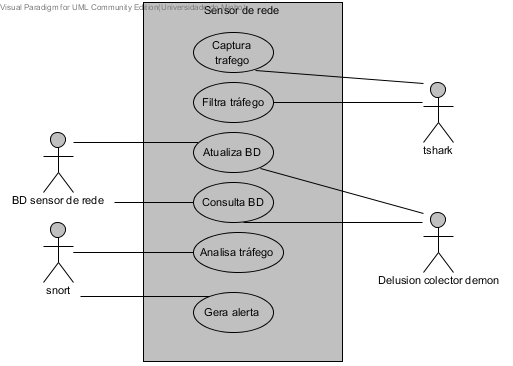
\includegraphics[scale=0.80]{images/ucs/Rede}
	\caption {Diagrama de use case, parte da Rede}
\end{figure}
\pagebreak

\newcommand{\uticomum}{\emph{utilizador comum}\xspace} 
\newcommand{\admini}{\emph{administrador}\xspace} 
\newcommand{\visualz}{\emph{visualizador}\xspace}
\subsubsection{\textbf{3 - Visualizador}}

Como já foi referido anteriormente (sec~\ref{sec: olare}) existem dois tipos de utilizadores: o \uticomum; e o \admini.\\ 

O \admini terá a mesma interacção com o \visualz que o \uticomum tem (que será explicado mais adiante), mais uma responsabilidade acrescida, 
conforme se pode ver na Figura~\ref{fig: casodeusovisual}:

\begin{itemize}
 \item \textbf{Configurar utilizadores} - esta funcionalidade diz respeito à gestão de utilizadores e engloba acções do tipo adicionar/remover utilizadores, 
 alterar permissões (por exemplo: acesso a configurações, tipos de visualizações permitidas, etc). A sua explicação estará mais detalhada em~\ref{subsubsec: confighoney} - 6.
\end{itemize}

O \uticomum terá como interacção com o sistema as seguintes funcionalidades:

\begin{itemize}
 \item \textbf{Ver Tráfego} - a funcionalidade que diz respeito a todas as formas de visualização que serão disponibilizadas pelo \visualz. Maioritariamente, a informação será exibida através de gráficos (de diversos tipos) e tabelas.
 \item \textbf{Ver Alertas} - os alertas que serão processados pelo \visualz, tanto poderão dizer respeito ao \emph{honeypot} como à rede.
 \item \textbf{Aplicar Filtros} - o utilizador poderá aplicar filtros às suas pesquisas, de modo a focalizar a informação ao que realmente lhe interessa.
 \item \textbf{Configurar Rede} - esta funcionalidade diz respeito às configurações que o utilizador poderá fazer à rede. A sua explicação estará mais detalhada em~\ref{subsubsec: confighoney} - 5.
 \item \textbf{Configurar Honeypot} - Finalmente, o utilizador poderá também configurar o \emph{honeypot}. A sua explicação estará mais detalhada em~\ref{subsubsec: confighoney} - 4.
\end{itemize}

\begin{figure}[!ht]
	\centering
	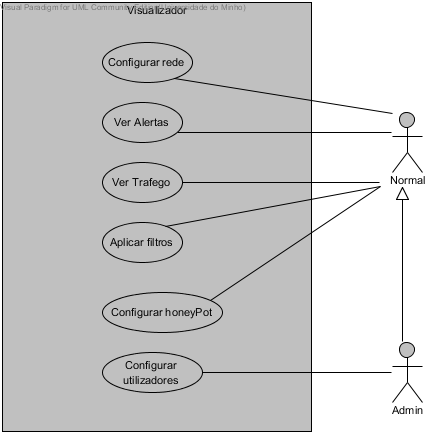
\includegraphics[scale=0.80]{images/ucs/Visualizador}
	\caption {Diagrama de use case, parte da Rede}~\label{fig: casodeusovisual}
\end{figure}
\pagebreak

\subsubsection{\textbf{4 - Configuração HoneyPot}}~\label{subsubsec: confighoney}

Uma das funcionalidades disponíveis na interação utilizador-\visualz, é a configuração do \emph{honeypot} (ver Figura~\ref{fig: confighoney}).
Esta funcionalidade está divida em três acções que o utilizador poderá tomar, sendo essas acções:

\begin{itemize}
 \item \textbf{Indicar SO} - através desta funcionalidade, o utilizador poderá indicar qual o sistema operativo que pretende virtualizar, indicando também certos parâmetros de \emph{hardware} da máquina.
 \item \textbf{Indicar serviços activos} - o utilizador poderá configurar, através do \visualz, quais os serviços activos que o \emph{honeypot} terá. Por exemplo, ter ou não activo um servidor \emph{apache}.
 \item \textbf{Indicar vulnerabilidades} - finalmente, o utilizador poderá também configurar certas vulnerabilidades nos serviços activos do \emph{honeypot}.
\end{itemize}

\begin{figure}[!ht]
	\centering
	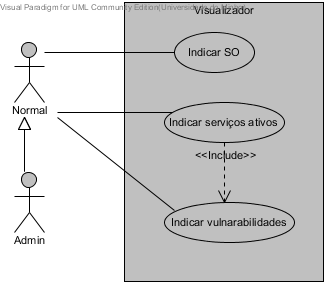
\includegraphics[scale=0.80]{images/ucs/ConfHoneyPot}
	\caption {Diagrama de use case, configuração HoneyPot}~\label{fig: confighoney}
\end{figure}
\pagebreak

\subsubsection{\textbf{5 - Configuração Rede}}
Como se pode ver na Figura~\ref{fig: confrede}, o utilizador poderá, caso tenha permissões para isso, configurar certas ferramentas que actuam sobre a rede. Desse modo, tem-se:

\begin{itemize}
 \item \textbf{Configurar IpTables} - configurar \emph{iptables}, será ...
 \item \textbf{Configurar Snort} - a configuração do \emph{Snort} passa por indicar parâmetros que irão influenciar na captura de pacotes ...
 \item \textbf{Configurar Tshark} - a configuração do \emph{Tshark} permitirá fazer alterações que influenciam o comportamento do mesmo, à semelhança do \emph{Snort}.
 \item \textbf{Configurar Rede} - esta funcionalidade diz respeito aos diversos parâmetros restantes que se podem modificar na rede. Tem-se como exemplo, a configuração de ...
\end{itemize}

\begin{figure}[!ht]
\centering
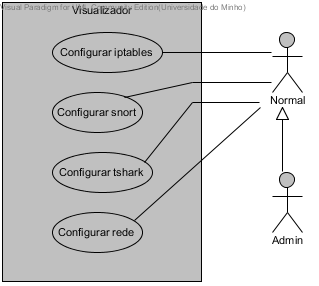
\includegraphics[scale=0.80]{images/ucs/ConfRede}
\caption {Diagrama de use case, configuração Rede}~\label{fig: confrede}.
\end{figure}
\pagebreak

\subsubsection{\textbf{6 - Configuração Utilizadores}}
Como na maioria dos sistemas de \emph{software}, haverá um controlo/gestão de utilizadores por parte de um ou mais \emph{administradores}. Assim, cabe ao \admini fazer essa gestão a partir das seguintes funcionalidades, consoante se pode ver na Figura~\ref{fig: confutil}:

\begin{itemize}
 \item \textbf{Criar Utilizador} - esta acção permite ao \admini criar um utilizador, indicando também certas propriedades que este irá ter, como por exemplo: se será o novo ultizador um \admini ou um \uticomum, se poderá ter permissões para configurar a rede/\emph{honeypot}, etc.
 \item \textbf{Editar Utilizador} - a partir desta acção, o \admini poderá alterar certas propriedade de um utilizador que foram, ou não, definidas aquando a sua criação.
 \item \textbf{Remover Utilizador} - finalmente, o \admini poderá eliminar utilizadores. A eliminação de um utilizador poderá implicar também a eliminação de outros registos.
\end{itemize}

\begin{figure}[!ht]
\centering
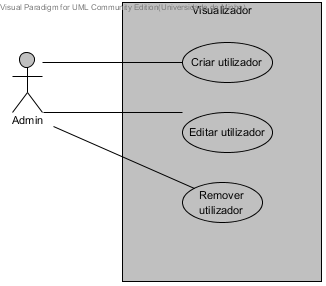
\includegraphics[scale=0.80]{images/ucs/ConfUtilizadores}
\caption {Diagrama de use case, configuração Utilizadores}~\label{fig: confutil}
\end{figure}
\pagebreak


\pagebreak
\section{Requisitos Funcionais}
De seguida apresentamos todos os requisitos funcionais do projecto. Apresentamos numa escala de 1 a 5 o nivel de prioridade, sendo 1 o mais baixo e 5 o mais alto.

\begin{minipage}{0.55\textwidth}
\begin{flushleft}\textbf{Requirement \#: 1}\end{flushleft}
\end{minipage}
\begin{minipage}{0.4\textwidth}
\end{minipage}

\begin{description}
\item \textbf{Description}:

O Qemu deve poder identificar chamadas do sistema e seu contexto, de forma automática. \\

\item \textbf{Rationale}:

Uma vez que o utilizador malicioso irá usar a máquina virtual, para seu proveito, é imperativo que seja registado
tudo o que ele faça no sistema. Umas das formas de registo será esta de identificar system calls e o contexto em que são chamadas,
nomeadamente id do processo, id do utilizador, e argumentos das system calls.

\item \textbf{Fit Criterion}:

\textbf{Todas} as system calls chamadas pelo guest OS, bem como, respectivos pid,uid e argumentos tem que ser registadas numa tabela. 

\item \textbf{Priority}:

5 em 5

\end{description}

\pagebreak


% Fim do requisito 









% Início do requisito 


\begin{minipage}{0.55\textwidth}
\begin{flushleft}\textbf{Requirement \#: 2}\end{flushleft}
\end{minipage}
\begin{minipage}{0.4\textwidth}
\end{minipage}

\begin{description}
\item \textbf{Description}:

O Qemu deve poder filmar as acções do utilizador malicioso, disponibilizando de seguida, o ficheiro respectivo em formato vídeo.\\


\item \textbf{Rationale}:

Como mais valia para o projecto, e como alternativa ao modo de visualização estático, o utilizador poderá ver de forma, mais "leve" o que
se passa no guest OS, proporciando-se, assim, uma maior maior eficiência na análise do ocorrido.


\item \textbf{Fit Criterion}:

Tem que ser possível ver um filme (sequência de capturas de ecrã) do guest OS, através de um ficheiro em formato vídeo,
para cada sessão que um utilizador malicioso tenha iniciado.

\item \textbf{Priority}:

2 em 5

\end{description}

\pagebreak


% Fim do requisito 


% Início do requisito 


\begin{minipage}{0.55\textwidth}
\begin{flushleft}\textbf{Requirement \#: 3}\end{flushleft}
\end{minipage}
\begin{minipage}{0.4\textwidth}
\end{minipage}

\begin{description}
\item \textbf{Description}:

O Qemu pode copiar qualquer ficheiro, que tenha sido interagido pelo utilizador malicioso, para o sistema onde está em funcionamento, 
ou, para um sistema remoto.

\item \textbf{Rationale}:

Por si só o registo de system calls é suficiente para registar os eventos iniciados pelo utilizador malicioso. Poderá no entanto haver casos
em que este faz um download de um ficheiro malicioso (onde detectar system calls pouco nos ajuda para analisar o que está presente no ficheiro), ou 
altera/cria ficheiros de texto. Nestes casos seria muito útil poder fazer uma cópia desses ficheiros para outro sistema para uma posterior análise.

\item \textbf{Fit Criterion}:

O Qemu ser capaz de transferir qualquer ficheiro para o Host ou mesmo para um sistema remoto.

\item \textbf{Priority}:

4 em 5

\end{description}

\pagebreak


% Fim do requisito 



% Início do requisito 


\begin{minipage}{0.55\textwidth}
\begin{flushleft}\textbf{Requirement \#: 4}\end{flushleft}
\end{minipage}
\begin{minipage}{0.4\textwidth}
\end{minipage}

\begin{description}
\item \textbf{Description}:

O daemon collector do Delusion (DCD), deve poder capturar qualquer tipo de trâfego que passe pela máquina virtual.

\item \textbf{Rationale}:

Até agora só foi falado de fazer registos de eventos após sessão iniciada pelo utilizador malicioso. No entanto, é muito importante
que o sistema seja capaz de registar todos os eventos a partir de que o utilizador tente interagir com a máquina virtual. Coisa que não é por si 
só possível com os requisitos anteriores.

\item \textbf{Fit Criterion}:

\textbf{Todo} o tráfego que passa pela máquina virtual tem que ser passível de ser registado, seja no sistema local ou num remoto.

\item \textbf{Priority}:

5 em 5

\end{description}

\pagebreak


% Fim do requisito 

% Início do requisito 


\begin{minipage}{0.55\textwidth}
\begin{flushleft}\textbf{Requirement \#: 5}\end{flushleft}
\end{minipage}
\begin{minipage}{0.4\textwidth}
\end{minipage}

\begin{description}
\item \textbf{Description}:

O utilizador consegue ver alertas, gerados pelo DCD, num browser.

\item \textbf{Rationale}:

O requisito anterior apesar de capturar toda a informação é demasiado verbosa para o utilizador. Se o sistema conseguir detectar padrões no 
trafego e avisar o utilizador desses padrões a detecção de eventos malignos será muito mais eficiente.

\item \textbf{Fit Criterion}:

Para um conjunto de tipo de ataques previamente definidos pelos utilizador. O sistema tem que ser capaz de conseguir detectar o padrão respectivo
a cada um deles e gerar um alerta.

\item \textbf{Priority}:

4 em 5

\end{description}

\pagebreak


% Fim do requisito 

% Início do requisito 


\begin{minipage}{0.55\textwidth}
\begin{flushleft}\textbf{Requirement \#: 6}\end{flushleft}
\end{minipage}
\begin{minipage}{0.4\textwidth}
\end{minipage}

\begin{description}
\item \textbf{Description}:

O utilizador consegue ver o trâfego que passou na máquina, capturado pelo DCD, num browser.

\item \textbf{Rationale}:
Para efeitos de simplicidade é extremamente útil que toda a informação respectiva ao trâfego convirga, de modo que, o utilizador 
não tenha que andar a analisar vários ficheiros distribuídos pelo sistema.

\item \textbf{Fit Criterion}:
Toda o trâfego coletado pelo sistema,tem que estar presente num ponto comum.

\item \textbf{Priority}:

4 em 5

\end{description}

\pagebreak


% Fim do requisito 


% Início do requisito 


\begin{minipage}{0.55\textwidth}
\begin{flushleft}\textbf{Requirement \#: 7}\end{flushleft}
\end{minipage}
\begin{minipage}{0.4\textwidth}
\end{minipage}

\begin{description}
\item \textbf{Description}:

O utilizador configurar os parâmetros de rede do HoneyPot, através dum browser.

\item \textbf{Rationale}:

Mais uma vez as ferramentas de configuração de redes, devem convergir numa só, de modo a que o utlizador não tenha que usar várias ferramentas
ao mesmo tempo, promovendo assim mais uma vez a simplicidade

\item \textbf{Fit Criterion}:

As ferramentas necessárias para configuração de rede do HoneyPot, tem que estar disponíveis a partir do visualizador.

\item \textbf{Priority}:

4 em 5

\end{description}

\pagebreak


% Fim do requisito 


% Início do requisito 


\begin{minipage}{0.55\textwidth}
\begin{flushleft}\textbf{Requirement \#: 8}\end{flushleft}
\end{minipage}
\begin{minipage}{0.4\textwidth}
\end{minipage}

\begin{description}
\item \textbf{Description}:

O utlizador consegue filtrar a informação, referente a eventos, através dum browser.

\item \textbf{Rationale}:

É importante que a informação consiga ser filtrada pelo utilizador, já que, este permite um maior foco na parte que o utilizador está
interessado, aumentando assim a produtividade da análise pretendida.

\item \textbf{Fit Criterion}:

A informação tem que ser possível de ser filtrada pelo visualizador, através de critérios definidos pelo utilizador.

\item \textbf{Priority}:

4 em 5

\end{description}

\pagebreak


% Fim do requisito 


% Início do requisito 


\begin{minipage}{0.55\textwidth}
\begin{flushleft}\textbf{Requirement \#: 9}\end{flushleft}
\end{minipage}
\begin{minipage}{0.4\textwidth}
\end{minipage}

\begin{description}
\item \textbf{Description}:

O utlizador consegue, escolher o tipo de gráfico usado para representar o trâfego e alertas, através dum browser.

\item \textbf{Rationale}:

Um conjunto de gráficos à escolha permite ao utilizador escolher o gráfico que mais se adequa ao tipo de informação e ao tipo de análise feita,
originando-se assim uma representação mais adequada à informação presente.


\item \textbf{Fit Criterion}:

A informação tem que ser possível de ser representada a partir de um gráfico previamente escolhida pelo utilizador.

\item \textbf{Priority}:

4 em 5

\end{description}

\pagebreak


% Fim do requisito 


% Início do requisito 


\begin{minipage}{0.55\textwidth}
\begin{flushleft}\textbf{Requirement \#: 10}\end{flushleft}
\end{minipage}
\begin{minipage}{0.4\textwidth}
\end{minipage}

\begin{description}
\item \textbf{Description}:

O utilizador consegue, configurar uma ou mais instâncias do HoneyPot, através dum browser.

\item \textbf{Rationale}:

No projecto, não é nosso interesse que o tipo de vulnerabilidade do sistema seja sempre o mesmo. É sim do nosso interesse que possamos criar
máquinas com vulnerabilidades diferentes permitindo assim uma melhor selecção dos utilizadores maliciosos a usar a máquina. Também é do nosso interesse
criar máquinas com características diferentes, por exemplo: arquitecturas, periféricos, memória RAM, etc..... Com isto cada máquina poderá ser adaptada
a cada situação pretendida.

\item \textbf{Fit Criterion}:

Tem que ser possível configurar os vários parâmetros de instâncias do HoneyPot, através de um browser

\item \textbf{Priority}:

4 em 5

\end{description}

\pagebreak


% Fim do requisito 


% Início do requisito 


\begin{minipage}{0.55\textwidth}
\begin{flushleft}\textbf{Requirement \#: 11}\end{flushleft}
\end{minipage}
\begin{minipage}{0.4\textwidth}
\end{minipage}

\begin{description}
\item \textbf{Description}:

O administrador consegue criar e remover utilizadores, através dum browser.


\item \textbf{Rationale}:
Não queremos que os utilizadores que podem aceder ao visualizador sejam fixos. Pode existir um futuro (muito provavelmente) onde irá ser preciso
uma pessoa para monitorar o HoneyPot, ou então seja preciso remover uma pessoa dessa monitorização. Posto isto será muito importante poder adicionar
ou remover utilizadores conforme necessário.

\item \textbf{Fit Criterion}:

O administrador poder criar ou remover utilizadores.

\item \textbf{Priority}:

5 em 5

\end{description}

\pagebreak


% Fim do requisito 


% Início do requisito 


\begin{minipage}{0.55\textwidth}
\begin{flushleft}\textbf{Requirement \#: 12}\end{flushleft}
\end{minipage}
\begin{minipage}{0.4\textwidth}
\end{minipage}

\begin{description}
\item \textbf{Description}:

O administrador gerir as permissões de utilizadores, através dum browser.


\item \textbf{Rationale}:

Como todos os utilizadores não são os mesmos, podemos querer dar acessos a algumas partes do HoneyPot a uns e negar o acesso a outros, para que isso aconteca é imperativo que haja um sistema de permissões que permita dar níveis de permissão a cada utilizador.

\item \textbf{Fit Criterion}:

O administrador tem que conseguir alterar as permissões de cada utilizador.

\item \textbf{Priority}:

4 em 5

\end{description}

\pagebreak


% Fim do requisito 


\chapter{Requisitos Não-Funcionais}
\minitoc
\section{Requisitos de Aspecto e Percepção}
\subsection{Requisitos de Estilo}
\begin{description}
\item[Requisito] O produto deve ter uma aparência profissional.
\item[Fit Criterion] Opinião favorável de todos os criadores do produto.
\end{description}

\section{Requisitos Humanos e Usabilidade}
\subsection{Requisitos de Usabilidade}
\begin{description}
\item[Requisito] O produto não deve ser aborrecido ou maçador de usar.
\item[Fit Criterion] Não abusar no uso de cores muito brilahntes, tamanho de letra sempre igual.
\end{description}

\section{Requisitos de Aprendizagem}
\begin{description}
\item[Requisito] Um administrador de redes familiarizado com Linux e ficheiros log deve conseguir utilizar o produto facilmente.
\item[Fit Criterion] Um grupo de pessoas que já fizeram administração de redes devem conseguir ambientar-se ao front-end no espaço de uma hora.
\end{description}

\section{Requisitos de Performance}
\subsection{Requisitos de Velocidade e Latência}
\begin{itemize}
\item A consulta da informação guardada não deverá demorar mais que 10 segundos.
\item A aplicação de filtros até encontrar a informação que se pretende não deverá demorar mais que 10 minutos.
\end{itemize}

\subsection{Requisitos de Precisão}
\begin{itemize}
\item O relógio do sistema trabalhará em GMT.
\end{itemize}

\subsection{Requisitos de Fiabilidade e Disponibilidade}
\begin{itemize}
\item O produto deverá funcionar sem falhas inesperadas em 99 de 100 utilizações.
\end{itemize}

\subsection{Requisitos de Longevidade}
\begin{itemize}
\item É esperado que o produto desempenhe a sua função correctamente de forma constante, até que a regulamentação da área de domínio que rege o seu funcionamento seja alterada.
\end{itemize}

\section{Requisitos Operacionais e Ambientais}
\subsection{Ambiente Físico Esperado}
\begin{itemize}
\item É esperado que este produto seja instalado numa rede num ambiente de uma empresa, dentro de um espaço fechado com ar condicionado e sistemas contra falhas de energia.
\end{itemize}

\subsection{Requisitos de Interacção com Sistemas Adjacentes}
\begin{description}
\item[Requisito] Este produto deverá ser utilizável nos quatro \emph{browsers} mais populares.
\item[Fit Criterion] O produto deveria ser utilizado com sucesso em acessos via Internet Explorer, Firefox, Google Chrome e Safari actualmente.
É expectável que estes continuem os quatro \emph{browsers} mais populares aquando da data de lançamento dos protótipos.
\end{description} 

\section{Requisitos de Manutenção e Suporte}
\subsection{Requisitos de Manutenção}
\begin{description}
\item[Requisito] O produto deve poder ser mantido por utilizadores e \emph{developers} que não os originais.
\item[Fit Criterion] O produto deve ser auto-suficiente em termos de suporte para utilizadores e \emph{developers} alheios ao desenvolvimento do produto, com recurso apenas ao manual de utilização.
\end{description}

 %done
\section{Requisitos de segurança}
Neste item iremos esclarecer alguns pontos relacionados com as questões de acesso, autorização, permissões e privacidade nos acessos aos dados do sistema. 

\textbf{Acesso}
As questões a nível de acesso físico ao servidor terão que ser tratadas com a empresa tomadora do produto e analisados caso a caso consoante também os recursos humanos que a empresa terá para lidar com a sua infra-estrutura tecnológica.
Contudo, genericamente, podemos dizer que o acesso físico ao servidor deverá somente ser feito ou autorizado pelo director dos sistemas de informação ou responsável pelo departamento informático, podendo incluir, nomeadamente:

\begin{itemize}
\item Administrador do sistema
\item Técnicos, nomeadamente para manutenção
\end{itemize}

Relativamente aos dados em si, existem algumas restrições no acesso e visualização dos mesmos, nomeadamente:
\begin{itemize}
\item Cada cliente só deverá ter acesso à sua própria informação
\item Cada mediador só deverá ver os dados dos seus clientes
\item O colaborador gere somente a configuração de produtos e fórmulas
\item O administrador do sistema terá acesso à globalidade da informação
\end{itemize}

\textbf{Integridade}
O bom funcionamento do sistema está dependente do bom funcionamento deste a nível aplicacional e a nível do sistema de informação. Assim são enumeradas algumas medidas a levar em consideração para assegurar esse bom funcionamento:
\begin{itemize}
\item Integridade da rede e comunicações, evitando assim acessos não autorizados
\item Incluir, se possível alguma redundância a nível de servidores de modo a aumentar a segurança da disponibilidade do serviço.
\item Incluir a nova aplicação no sistema de backups da empresa, nomeadamente a base de dados.
\end {itemize}

A nível de funcionamento aplicacional serão também tidos alguns cuidados de modo a aumentar a coerência dos dados inseridos, designadamente a validação dos dados recolhidos pela aplicação para que estes estejam de acordo com o modelo do sistema de informação.

\textbf{Privacidade}
O sistema informará o cliente que todos os dados armazenados serão confidenciais e não disponibilizados a terceiros para outro tipo de tratamento que não o inerente ao funcionamento do sistema em si.
Qualquer alteração nesta politica de funcionamento será atempadamente comunicada ao cliente e terá que ter a concordância deste.
Os dados armazenados seguirão as normas e directrizes dadas pelo sistema nacional de protecção de dados bem.

\textbf{Auditoria}
O sistema operativo poderá guardar informação relevante para uma auditoria ao funcionamento da aplicação, no entanto a nível interno, o sistema poderá guardar histórico de informação inserida, alterada ou removida para facilitar um processo de auditoria ao funcionamento da aplicação.

\textbf{Imunização}
A aplicação não prevê qualquer tipo de protecção adicional no que diz respeito a possíveis ataques de programas não autorizados ou indesejados, como sendo infecções de sistema por viroses, cavalos de tróia entre outros. A protecção é dada pelos acessos autorizados dos utilizadores à aplicação, quaisquer outras considerações terão que ser previstas no conjunto de protecções necessárias às máquinas que alojam os sistemas aplicionais e de informação e à própria rede em si.

\section{Requisitos culturais e políticos}
\subsection{Requisitos culturais}
Nesta secção serão apresentação os requisitos específicos relacionados com os factores sociológicos que afectam a aceitabilidade do produto.
\begin{itemize}
\item O produto não deverá ser ofensivo para os grupos étnicos e religiosos do pais de origem.
\item O produto deverá ser capaz de distinguir diferentes línguas e também diferentes sistemas de numeração, consoante o país de origem.
\item O produto deverá registar os feriados públicos do país.
\item O produto deverá se adaptar ao ambiente cultural do país, evitando símbolos, palavras e cores ofensivas para a sua cultura.
\end{itemize}

\subsection{Requisitos políticos}
Esta secção contém requisitos específicos relacionados com factores políticos que afectam a aceitabilidade do produto.
\begin{itemize}
\item O produto deverá fornecer todas as funcionalidades ao administrador da empresa (CEO).
\end{itemize}

\section{Requisitos Legais}
\subsection{Requisitos de conformidade}

Esta secção refere os requisitos legais do produto.
\begin{itemize}
\item O produto deverá ir de encontro à legislação em vigor no país.
\item O produto deverá respeitar a propriedade intelectual bem como os direitos de autor.
\item O produto deverá armazenar os dados seguirão as normas e directrizes dadas pelo sistema nacional de protecção de dados.
\end{itemize}

 %done
\chapter{Questões do Projecto}
\minitoc
\section{Pontos em aberto}
Relativamente a este projecto existem algumas questões importantes que necessitam de um esclarecimento prévio por parte do cliente.
A resposta a estas questões é essencial para o planeamento e para uma melhor especificação do sistema em si:

\subsection{Especificação entidades sistema}
Da análise prévia já efectuada, foram identificados intervenientes neste sistema:

\begin{itemize} 
\item Utilizador (anónimo/registado)
\item Administrador (empresa de seguros)
\item Mediador (Corretor/Agente/Mediador de seguros ligado)
\end{itemize}

É necessário especificar se existe mais alguma entidade a ser considerada que tenha interacção no sistema a desenvolver e quais as suas competências. Relativamente à entidade mediador esclarecer a divisão feita: Mediador em Corretor, Agente, e Mediador de Seguros Ligado (actualização do antigo estatuto de Angariador no Decreto-Lei n 144/2006, de 31 de Julho).

\subsection{Sistema por empresa}
Clarificar se a empresa de seguros necessita de implementar um sistema único para várias possíveis sucursais ou se a configuração é feita unitariamente sempre para cada empresa/sucursal.


\section{Novos Problemas}

\subsection{Incorporação aplicações}
Para aplicações actualmente existentes e sobre os quais terá que haver uma partilha ou transferência de dados terá também que ser efectuada uma análise, nomeadamente:

\begin{itemize} 
\item Identificação e levantamento aplicações sobre as quais haverá partilha ou fluxo de dados
\item Identificação dos dados a serem partilhados para cada aplicação
\item Definição de métodos e formatos de partilha de dados para cada aplicação
\item Definição de tarefas e calendarização  
\end{itemize} 

\subsection{Manutenção do sistema}
O seguimento do sistema, depois da sua instalação é assegurado por um serviço de suporte ao produto, disponibilizado pela empresa fornecedora do sistema. Contudo, esse suporte não cobre situações externas que possam influenciar o funcionamento deste, tais como problemas com infra-estrutura e comunicações, que terão que ser asseguradas pela empresa tomadora do sistema. 

\section{Tarefas}
\subsection{Planeamento}
Estão previstas as fases abaixo descritas, respectivas tarefas e resultados:
\begin{sidewaystable}[!p]
\begin{center}
\setlength{\tabcolsep}{5pt}
\begin{tabular}{|p{1cm}|p{1.2cm}|p{1.2cm}|p{1.2cm}|p{1.2cm}|p{1.2cm}|p{1.2cm}|p{1.2cm}|p{1.2cm}|p{2.4cm}|p{2.4cm}|}
\hline & \multicolumn{8}{|c|}{\T \B \textbf{Fases Iniciais}} & \multicolumn{1}{|c|}{\textbf{Formação}} & \multicolumn{1}{|c|}{\textbf{Suporte}}\\
\cline{2-9} & \multicolumn{2}{|c|}{\T \B \textbf{Concepção}} & \multicolumn{2}{|c|}{\textbf{Elaboração}} & \multicolumn{2}{|c|}{\textbf{Construção}} & \multicolumn{2}{|c|}{\textbf{Transição}} & \multicolumn{1}{|c|}{\textbf{ }} & \multicolumn{1}{|c|}{\textbf{ }}\\
\hline \multirow{6}{3cm}{\begin{sideways}\T \B \parbox{3cm}{Tarefas (Peso)}\end{sideways}} & MN & (+) & MN & (+) & MN & (o) & MN & (-) & & \\
\cline{2-9} & AR & (+) & AR & (+) & AR & (o) & AR & (-) & & \\
\cline{2-9} & ED & (*) & ED & (*) & ED & (+) & ED & (o) & Formação & Suporte \\
\cline{2-9} & IMP & (o) & IMP & (*) & IMP & (+) & IMP & (o) & (+) & (+)\\
\cline{2-9} & TST & (-) & TST & (o) & TST & (*) & TST & (+) & & \\
\cline{2-9} & INST & (-) & INST & (-) & INST & (-) & INST & (+) & & \\
\hline \multirow{5}{3cm}{\begin{sideways}\T \B \parbox{3cm}{Resultados}\end{sideways}} & \multicolumn{2}{|p{2cm}|}{Domínio do Sistema} & \multicolumn{2}{|p{2cm}|}{Descrição e Arquitectura do Sistema} & \multicolumn{2}{|p{2cm}|}{Protótipo do Sistema} & \multicolumn{2}{|p{2cm}|}{Migração, incorporação das aplicações existentes} & Formação dos Utilizadores & Suporte Aplicacional\\
\cline{2-11}\T \B & \multicolumn{2}{|p{2cm}|}{Identificação dos Stakeholders} & \multicolumn{2}{|p{2cm}|}{Descrição do negócio e riscos do projecto} & \multicolumn{2}{|p{2cm}|}{Validação} & \multicolumn{2}{|p{2cm}|}{Instalação} &  & Tarefas de manutenção do sistema\\
\cline{2-11}\T \B & \multicolumn{2}{|p{2cm}|}{Análise de Requisitos} & \multicolumn{2}{|p{2cm}|}{Plano de Desenvolvimento} & \multicolumn{2}{|p{2cm}|}{Testes} & \multicolumn{2}{|p{2cm}|}{Entrada em produção} & & Migrações\\
\cline{2-11}\T \B & \multicolumn{2}{|p{2cm}|}{Estimativa inicial de custos} & \multicolumn{2}{|p{2cm}|}{Especificação do sistema} & \multicolumn{2}{|p{2cm}|}{ } & \multicolumn{2}{|p{2cm}|}{ } & & \\
\cline{2-11}\T \B & \multicolumn{2}{|p{2cm}|}{Avaliação inicial de prioridades, riscos e processo de desenvolvimento} & \multicolumn{2}{|p{2cm}|}{Modelo da aplicação} & \multicolumn{2}{|p{2cm}|}{ } & \multicolumn{2}{|p{2cm}|}{ } & & \\
 \hline
\end{tabular}
 \caption{Tabela de Planeamento}
\end{center}
\end{sidewaystable}
\clearpage
\subsection{Prazos}
De seguida faz-se uma estimativa dos diferentes prazos para as fases acima expostas:

\begin{table}[!h]
\begin{center}
\setlength{\tabcolsep}{2pt}
\begin{tabular}{|p{1.5cm}|p{1.5cm}|p{1.5cm}|p{1.5cm}|p{1.5cm}|p{2.2cm}|p{2.2cm}|}
\hline & \multicolumn{4}{|c|}{\T \B \textbf{Fases Iniciais}} & \multicolumn{1}{|c|}{\textbf{Formação}} & \multicolumn{1}{|c|}{\textbf{Suporte}}\\
\cline{2-5} & \multicolumn{1}{|c|}{ \T \B \textbf{Concepção}} & \multicolumn{1}{|c|}{\textbf{Elaboração}} & \multicolumn{1}{|c|}{\textbf{Construção}} & \multicolumn{1}{|c|}{\textbf{Transição}} & \multicolumn{1}{|c|}{\textbf{ }} & \multicolumn{1}{|c|}{\textbf{ }}\\
\hline \T \B Data Limite & Janeiro 2010 & Fevereiro 2010 & Abril 2010 & Maio 2010 & A especificar & A especificar\\
 \hline
\end{tabular}
 \caption{Tabela de Prazos}
\end{center}
\end{table}

\section{Migração para o novo produto}
\subsection{Requisitos}
Para garantir a migração para o novo produto a empresa tomadora do produto terá que garantir algumas condições necessárias, nomeadamente:

\begin{itemize} 
\item Infra-estrutura: local adequado onde irá ser albergado o(s) servidor(es) que serviram de suporte ao sistema, com condições adequadas ao seu funcionamento.
\item Requisitos de hardware: fornecimento da máquina, ou máquinas onde serão instalados o servidor de base de dados e o servidor aplicacional.
\item Requisitos de software: fornecimento do software base de suporte aplicacional, onde se inclui por exemplo o sistema operativo, componentes necessários para o funcionamento do sistema e base de dados.
\end{itemize}

É necessário também incluir a nova aplicação no sistema de backups da empresa, quer a nível aplicacional como de dados.
Em caso de migração ou incorporação de aplicações existentes terá que haver uma análise caso a caso para análise dos requisitos necessários para efectivar essa mesma migração ou incorporação.
 
\section{Riscos}
Todos os projectos envolvem riscos. O risco não é necessariamente uma coisa má, pelo que, sem riscos não existe avanço nos projectos. No entanto, existem diferenças entre os riscos, ou seja, entre os riscos incontrolados e os riscos passíveis de ser geridos. Os riscos só são maus se forem ignorados e começarem a dar problemas.
A gestão de riscos implica a apreciação daqueles riscos que são mais prováveis de aplicar no projecto, decidindo o curso a tomar se esses riscos se tornarem problemas, e também na monitorização dos projectos de forma a detectar-se precocemente sinais sobre os riscos, de maneira a evitar que se tornem problemas.
Abaixo passamos a citar a lista dos riscos mais prováveis e mais sérios de aparecer no projecto. Cada risco incluiu uma probabilidade de ele se tornar um problema.

\begin{itemize}
\item \textbf{Mudança dos requisitos} 
Uma mudança nos requisitos acarreta um significativo risco no projecto, significando alterações na modelação dos requisitos iniciais. A probabilidade deste risco se tornar problema é alta, visto que não depende exclusivamente da equipa de desenvolvimento, e portanto, torna-se volátil a sua execução.

\item \textbf{Pressão excessiva do cronograma} 
O cronograma é um risco calculado que poderá se tornar problema quando se deixa de controlar o tempo. A probabilidade deste risco se tornar problema é relativamente baixa visto que todos os envolvidos no projecto estão cientes dos prazos a cumprir.

\item \textbf{Requisitos problemáticos do utilizador}
Por vezes os requisitos dos utilizadores tornam-se riscos para o projecto visto que muitos deles só são vistos como não exequíveis numa fase adiantada do projecto. A probabilidade de se tornar problema pode ser alta se os requisitos problemáticos não forem detectados inicialmente.

\item \textbf{Qualidade baixa}
O risco da qualidade do produto só será problema se o produto desenvolvido não corresponder ao expectável pelo cliente. No entanto, esse risco é controlável através dos diversos pontos de controlo do projecto ao longo do seu desenvolvimento. A probabilidade de se tornar um problema é baixa.
\end{itemize}

Tendo em conta a análise aos riscos envolvidos e considerando valores quantificáveis para as probabilidades desses riscos se tornarem problemas, apresenta-se abaixo uma estimativa para exposição ao risco.

\begin{table}[!h]
\begin{center}
\begin{tabular}{|p{3.5cm}|p{3.5cm}|p{4cm}|}
\hline \multicolumn{1}{|c|}{\T \B \textbf{Riscos}} & \multicolumn{1}{|c|}{\textbf{Probabilidade}} & \textbf{Estimativa = Probabilidade $\times$ Impacto}\\
\hline \T \B Mudança dos requisitos & Alta (valor 0,8) & $E(r) = 0,8 \times 8 = 6,4$\\
\hline \T \B Pressão excessiva do cronograma & Baixa (valor 0,1) & $E(r) = 0,1 \times 3 = 0,3$\\
\hline \T \B Requisitos problemáticos do utilizador & Alta (valor 0,8) & $E(r) = 0,8 \times 9 = 7,2$\\
\hline \T \B Qualidade baixa & Baixa (valor 0,1) & $E(r) = 0,1 \times 9 = 0,9$\\
\hline
\end{tabular}
 \caption{Tabela de Riscos}
\end{center}
\end{table}
\textbf{Impacto do risco}: Varia entre 1 e 10

\textbf{Probabilidade do risco}: Varia entre 0 e 1 (baixa, média e alta)
 
\section{Custos}
A duração global prevista para este projecto a ser efectuada por um recurso humano por dia é de seis meses. O custo dia de um recurso humano é de 50 euros. Sendo assim, o custo estimado para este projecto, considerando 21 dias úteis, é 12.600 euros. Assim serão admitidos ao projecto o número essencial de recursos humanos de forma a garantir a sua exequibilidade no prazo estipulado. 
Em relação à manutenção do sistema, será necessário contabilizar o custo de um administrador do sistema, pago de acordo com o valor de mercado.
Por fim acresce ao custo o valor da formação dada aos utilizadores do sistema. Esse custo é medido em função do número de horas praticadas.
Será ainda necessário comprar hardware no valor de 3.500 euros para suportar toda a estrutura do \textit{Delusion}.

\section{Documentação e formação do Utilizador}
\subsection{Documentação}
Neste projecto, fará parte a seguinte documentação:

\begin{itemize}
\item \textbf{Manual do utilizador} – Específica todas as funcionalidades do software, de forma simples e intuitiva, de maneira a ajudar os utilizadores na utilização do mesmo. Este manual será para uso de todos os utilizadores do sistema.

\item \textbf{Manual de administração} – Específica todas as tarefas necessárias para instalar e administrar o software. Refere também todos os recursos necessários ao nível de hardware e software de forma que o produto funcione sem problemas. Este documento será para uso exclusivo do administrador do sistema.
\end{itemize}

Esta documentação será elaborada por um subconjunto da equipa de desenvolvimento do projecto. A equipa será responsável também pela actualização da mesma. Toda a documentação será fornecida em formato digital (ficheiros pdf). 

\subsection{Formação dos utilizadores}
A formação dos utilizadores será numa primeira fase da responsabilidade de alguns dos engenheiros de software da equipa de desenvolvimento. Estes terão como responsabilidade ministrar acções de formação com os utilizadores do produto, de forma a instruir os utilizadores das principais funcionalidades do produto. Essas acções serão iniciadas após a instalação do produto. Estas acções de formação têm como finalidade envolver os utilizadores comuns do sistema no manuseamento do produto, de forma a torná-los autónomos da sua utilização.


\appendix
\chapter{Glossário}
\label{appendix:1}
\begin{description}
    \item \textbf{Autenticidade}

    Propriedade de segurança que tem como finalidade assegurar a “origem” da mensagem.
\end{description}

\begin{description}
    \item \textbf{Confidencialidade}

    Propriedade de segurança que tem como finalidade garantir que o conteúdo da mensagem só é do conhecimento de intervenientes legítimos.
\end{description}

\begin{description}
    \item \textbf{Firewall}

    Uma firewall é um dispositivo, ou um conjunto de dispositivos, que tem como função permitir ou negar certas transmissões de rede, protegendo desta forma o sistema onde está instalada. Numa rede em que esteja instalada uma \textit{Firewall} todas as ligações não autorizadas são bloqueadas, permitindo apenas ligações legítimas.
\end{description}

\begin{description}
    \item \textbf{Gateway}
    
    Um gateway é um nodo de uma rede que actua como um elo de ligação entre duas redes distintas.
\end{description}

\begin{description}
    \item \textbf{Honeypot}

    Um Honeypot é um serviço que é instalado numa rede com os seguintes objectivos:
    \begin{itemize}
        \item desviar a atenção dos atacantes de serviços mais sensíveis e importantes;
        \item perceber os ataques infligidos.
    \end{itemize}
    
    Os dados recolhidos durante o funcionamento de um \textit{Honeypot} auxiliam os administradores de sistema a proteger os serviços reais.\\
    
    Geralmente num Honeypot são colocados serviços cujas vulnerabilidades são conhecidas, de forma a atrair os atacantes para uma máquina que não possui informações importantes.
\end{description}

\begin{description}
    \item \textbf{Integridade}

    Propriedade de segurança que tem com finalidade garantir que o receptor não “aceita” mensagens que tenham sido manipuladas.
\end{description}

\begin{description}
    \item \textbf{Intrusion Detection System}
    
    Um sistema de detecção de intrusões (\textit{IDS}) é um dispositivo que monitoriza a rede, ou até as actividades de um dado sistema, em busca de actividades maliciosas ou de violações da política da rede imposta. O resultado desta monitorização é exportado através de \textit{logs}, para que mais tarde possa ser consultada pelos administradores de sistema.
\end{description}

\begin{description}
    \item \textbf{Máquina Virtual}
    
    Com uma Máquina Virtual consegue-se simular através de software o funcionamento de um computador real. Este funcionamento permite correr sistemas operativos como se fossem aplicações de outros sistemas operativos.\\

    O sistema operativo onde a máquina virtual corre é designado de \textit{host}.
    O sistema operativo que está a ser virtualizado é designado de \textit{guest}.
\end{description}

\begin{description}
    \item \textbf{Netflow}

O \textit{Netflow} é um protocolo da Cisco que colecciona informação de tráfego na rede. Esta ferramenta utiliza a nocção de \textit{network flow}, que consiste num conjunto de pacotes que partilham os mesmos endereços IP e portas de origem e destino, entre outros atributos, durante um determiado intervalo de tempo. 
\end{description}

\begin{description}
    \item \textbf{Nfcapd}

O \textit{Nfcapd}é uma ferramenta designada como um \textit{collector}, cujo objectivo é receber e agregar a informação de flows.
\end{description}

\begin{description}
    \item \textbf{Nmap}

   O \textit{NMap} é uma ferramenta gratuita e \textit{open-source} usada para explorar uma infraestrutura de rede, ou até em auditorias de segurança. Com o \textit{Nmap} é possível encontrar que sistemas operativos estão instalados, que serviços -- incluindo versões --  estão disponibilizados nas várias máquinas da rede.
\end{description}

\begin{description}
    \item \textbf{Qemu}

    O \textit{QEMU} é uma ferramenta \textit{open-source} que permite criar máquinas virtuais.
\end{description}

\begin{description}
    \item \textbf{Sniffer}
    Um \textit{Sniffer} tem como finalidade interceptar e registar o trâfego gerado numa rede. 
\end{description}

\begin{description}
    \item \textbf{Softflowd}

    Esta ferramenta é designada como um \textit{exporter}, cujo objectivo é monitorizar a rede e exportar a informação de flows.
\end{description}

\begin{description}
    \item \textbf{Snort}

    O Snort é um \textit{IDS (Intrusion Detection System) Open Source}. A sua função consiste em analisar o tráfego da rede em busca de possíveis ataques. Para isso, dispõe de uma base de dados de assinaturas de pacotes correspondentes a tráfego malicioso (chamadas regras). Esta base de dados é composta por regras criadas pelos utilizadores, com finalidades diferentes, como por exemplo: detectar IPs ou portas utilizadas, ou até análisar o payload dos pacotes.
\end{description}

\begin{description}
    \item \textbf{System Call}

    Uma \textit{System Call} é um serviço disponibilizado pelo sistema operativo às aplicações, para que estas consigam utilizar os vários elementos do computador, como por exemplo escrever ou ler a partir de um ficheiro.
\end{description}

\begin{description}
    \item \textbf{Router}

    Um router é um dispositivo que permite a ligação entre duas ou mais redes distintas.
\end{description}

\begin{description}
    \item \textbf{Tshark}
    O \textit{Tshark} é uma ferramenta utilizada para observar na linha de comandos os registos gerados pelo \textit{Wireshark}.
\end{description}

\begin{description}
    \item \textbf{Wireshark}

    O \textit{Wireshark} é uma ferramenta utilizada para interceptar e registar pacotes de rede.
\end{description}

\begin{description}
    \item \textbf{Web Service}
    
    Um \textit{Web Service} é um método de comunição entre dois dispositivos electrónicos através de uma rede.
\end{description}


%\chapter{\emph{Use Cases}}
%

\section{Simulador}
\begin{figure}[!htb]
	\centering
	\includegraphics[scale=0.8]{images/Prints/Simulador/Simulador.pdf}
\end{figure}

\pagebreak

\subsection{Simulação Uni/Multiproduto}
\begin{figure}[!htb]
	\centering
	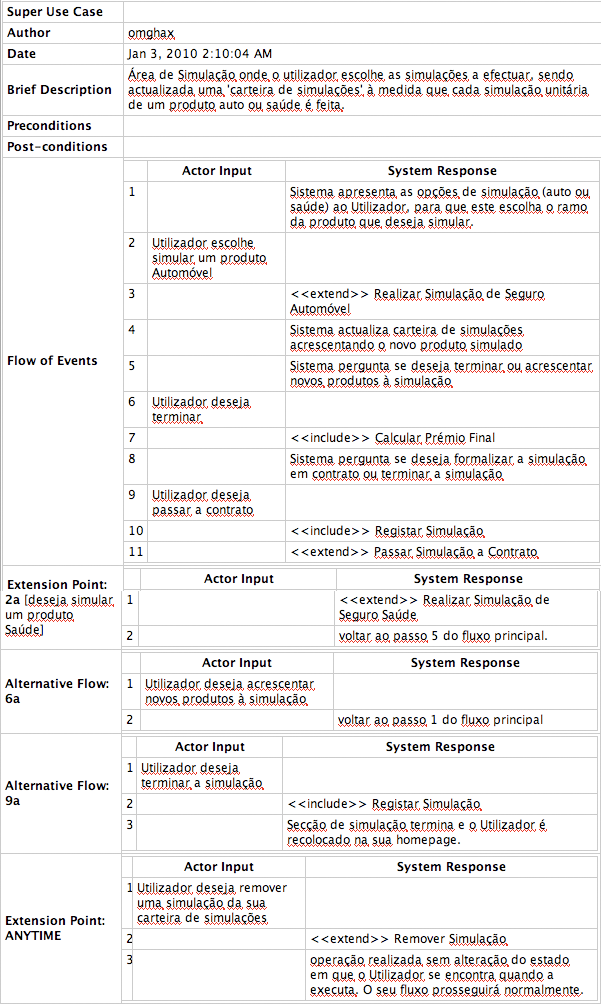
\includegraphics[scale=0.53]{images/Prints/Simulador/SimulacaoUniMultiproduto.png}
\end{figure}

\pagebreak

\subsection{Gestão da Simulação de Seguros}
\begin{figure}[!htb]
	\centering
	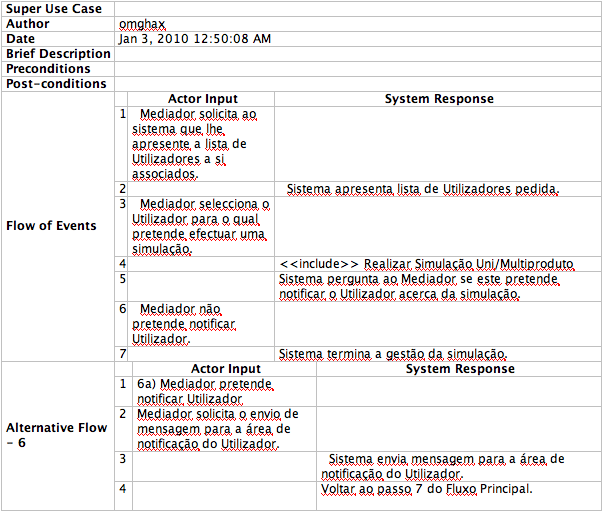
\includegraphics[scale=0.60]{images/Prints/Simulador/GerirSimulacaoSeguros.png}
\end{figure}

\subsection{Registo de Simulação}
\begin{figure}[!htb]
	\centering
	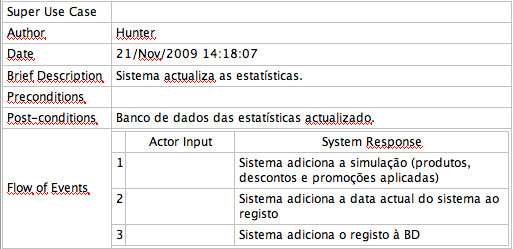
\includegraphics[scale=0.60]{images/Prints/Simulador/RegistarSimulacao.png}
\end{figure}

\pagebreak

\subsection{Remover Simulação}
\begin{figure}[!htb]
	\centering
	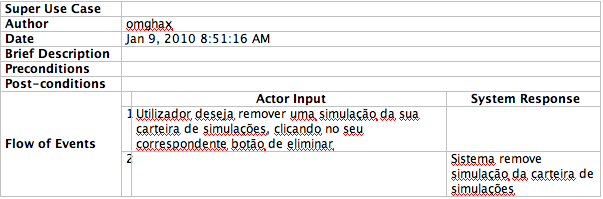
\includegraphics[scale=0.63]{images/Prints/Simulador/RemoverSimulacao.png}
\end{figure}

\subsection{Cálculo do Prémio Final}
\begin{figure}[!htb]
	\centering
	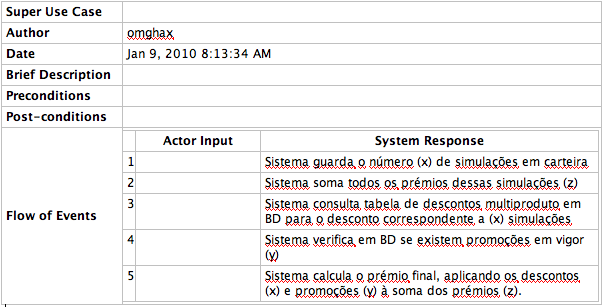
\includegraphics[scale=0.63]{images/Prints/Simulador/CalcularPremioFinal.png}
\end{figure}


\pagebreak

\section{Simulação Automóvel}
\begin{figure}[!htb]
	\centering
	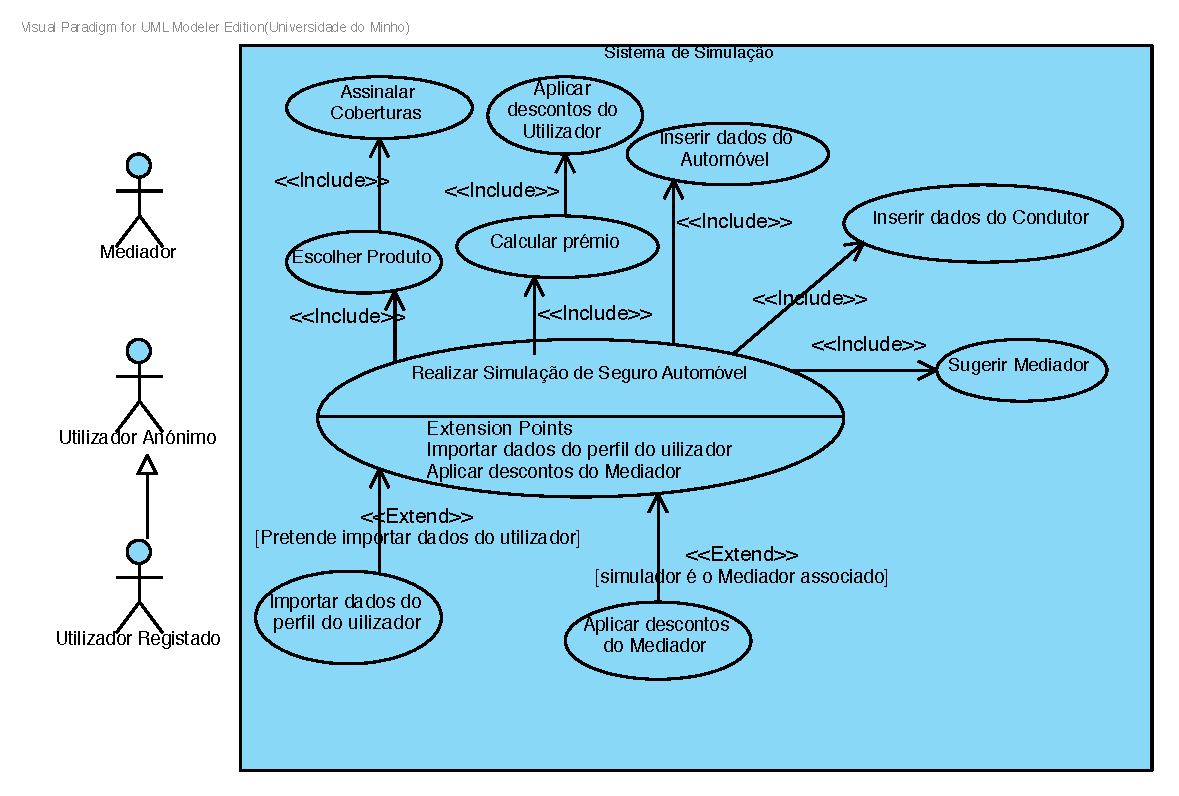
\includegraphics[scale=0.85]{images/Prints/RealizacaoSeguroAutomovel/SimulacaoSeguroAuto.pdf}
\end{figure}

\pagebreak

\subsection{Realizar Simulação de Seguro Automóvel}
\begin{figure}[!htb]
	\centering
	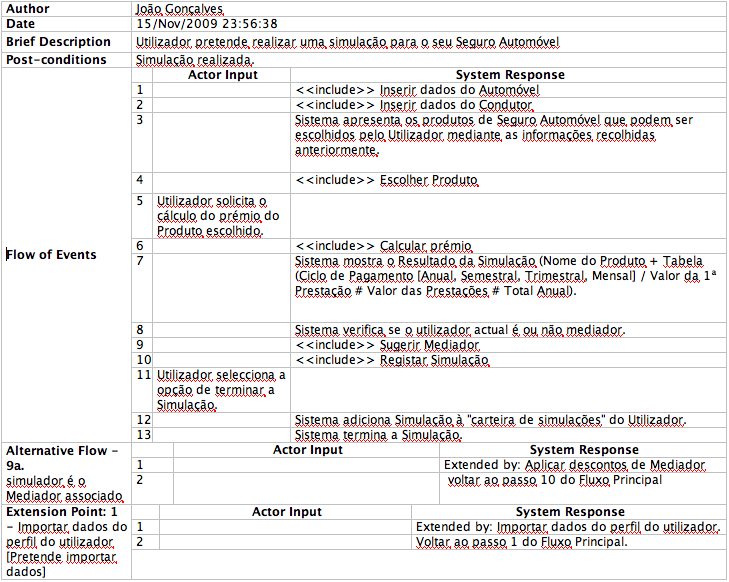
\includegraphics[scale=0.6]{images/Prints/RealizacaoSeguroAutomovel/RealizacaoSeguroAutomovel.png}
\end{figure}

\pagebreak

\subsection{Inserir dados do Condutor}
\begin{figure}[!htb]
	\centering
	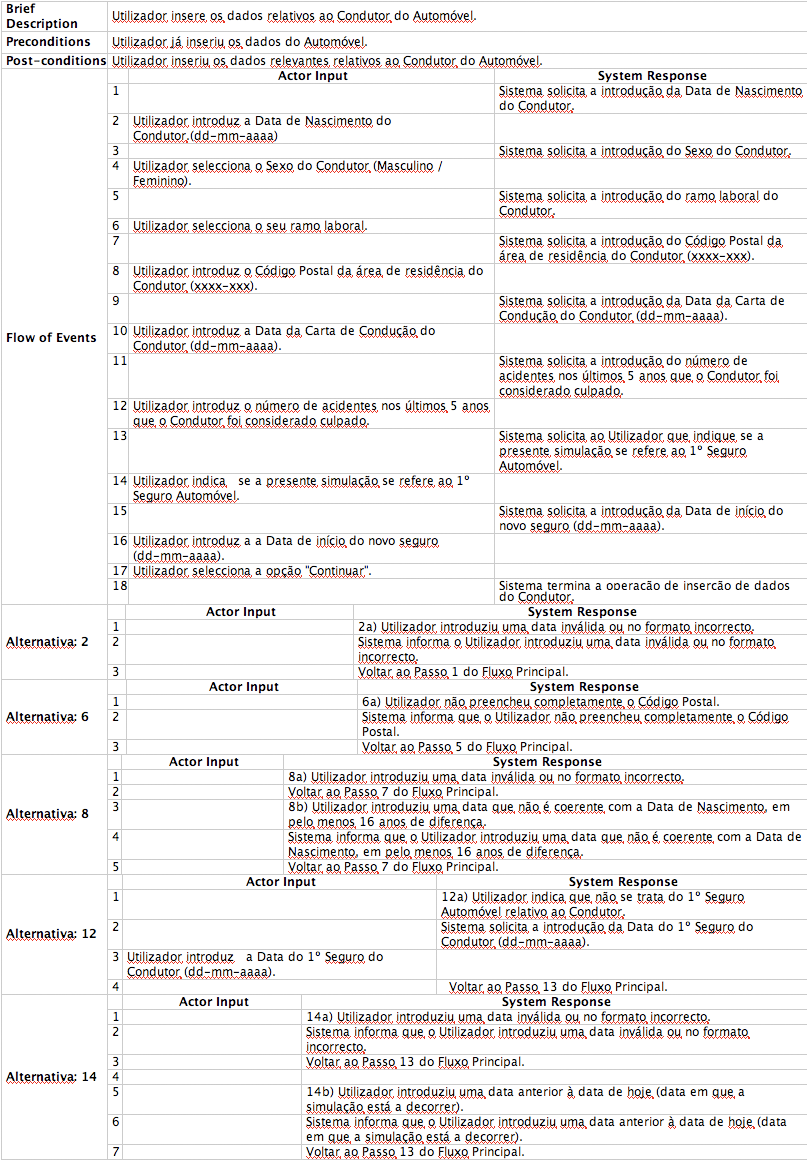
\includegraphics[scale=0.45]{images/Prints/RealizacaoSeguroAutomovel/InserirDadosDoCondutor.png}
\end{figure}

\pagebreak

\subsection{Inserir dados do Automóvel}
\begin{figure}[!htb]
	\centering
	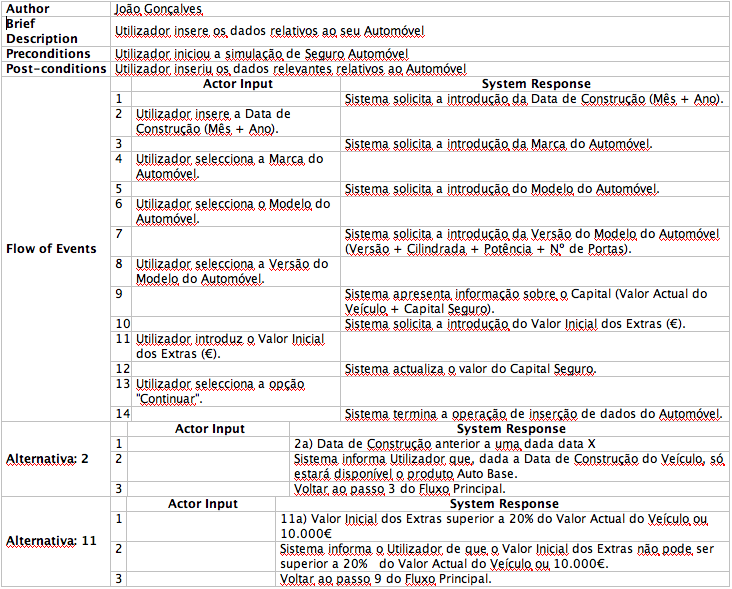
\includegraphics[scale=0.6]{images/Prints/RealizacaoSeguroAutomovel/InserirDadosAutomovel.png}
\end{figure}

\pagebreak

\subsection{Calcular prémio}
\begin{figure}[!htb]
	\centering
	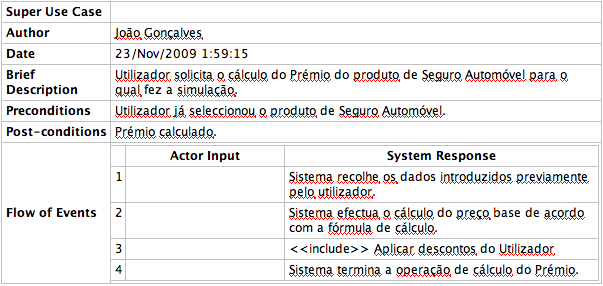
\includegraphics[scale=0.6]{images/Prints/RealizacaoSeguroAutomovel/CalcularPremio.png}
\end{figure}

\subsection{Aplicar descontos do Utilizador}
\begin{figure}[!htb]
	\centering
	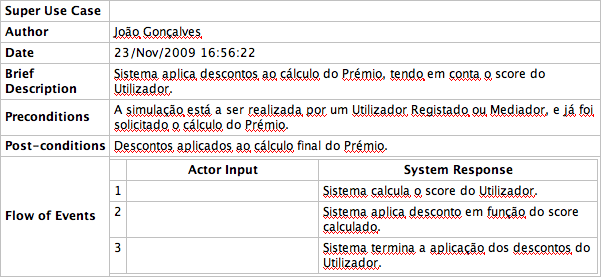
\includegraphics[scale=0.7]{images/Prints/RealizacaoSeguroAutomovel/AplicarDescontosUtilizador.png}
\end{figure}

\pagebreak

\subsection{Escolher Produto}
\begin{figure}[!htb]
	\centering
	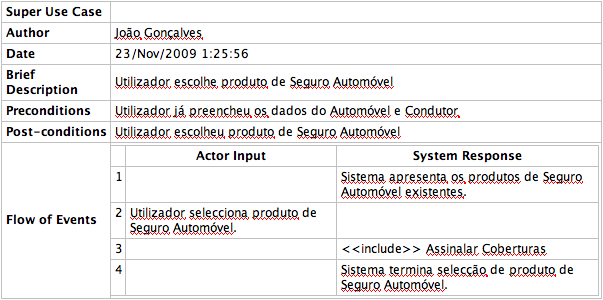
\includegraphics[scale=0.7]{images/Prints/RealizacaoSeguroAutomovel/EscolherProduto.png}
\end{figure}

\subsection{Assinalar Coberturas}
\begin{figure}[!htb]
	\centering
	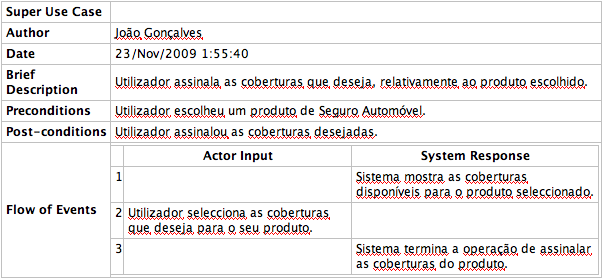
\includegraphics[scale=0.7]{images/Prints/RealizacaoSeguroAutomovel/AssinalarCoberturas.png}
\end{figure}

\pagebreak

\subsection{Sugestão de mediador}
\begin{figure}[!htb]
	\centering
	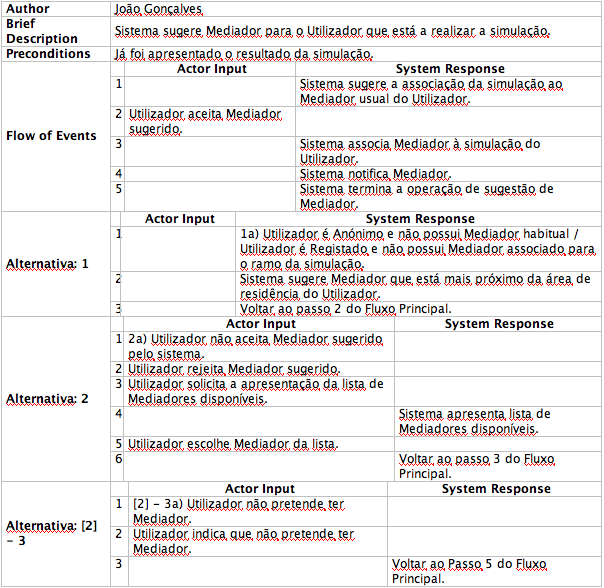
\includegraphics[scale=0.72]{images/Prints/RealizacaoSeguroAutomovel/SugerirMediador.png}
\end{figure}

\pagebreak

\subsection{Aplicar o Desconto de Mediador}
\begin{figure}[!htb]
	\centering
	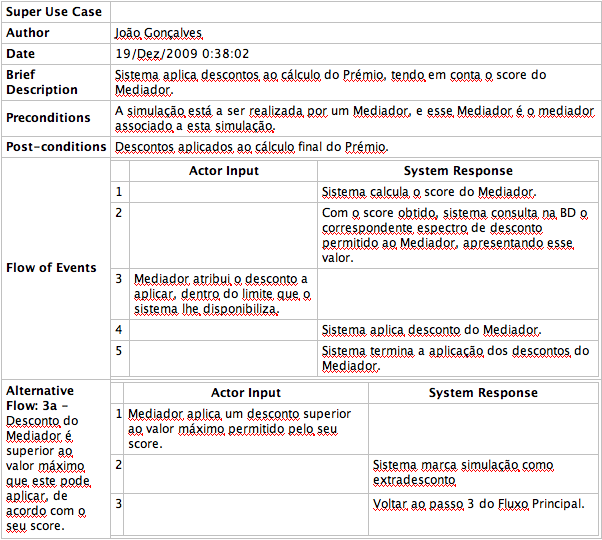
\includegraphics[scale=0.69]{images/Prints/RealizacaoSeguroAutomovel/AplicarDescontosMediador.png}
\end{figure}

\pagebreak

\subsection{Importar dados do Utilizador}
\begin{figure}[!htb]
	\centering
	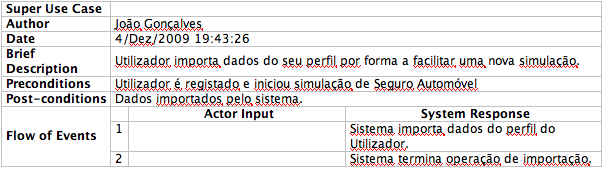
\includegraphics[scale=0.70]{images/Prints/RealizacaoSeguroAutomovel/ImportarDadosPerfilUtilizador.png}
\end{figure}


\section{Simulação Saúde}
\begin{figure}[!htb]
	\centering
	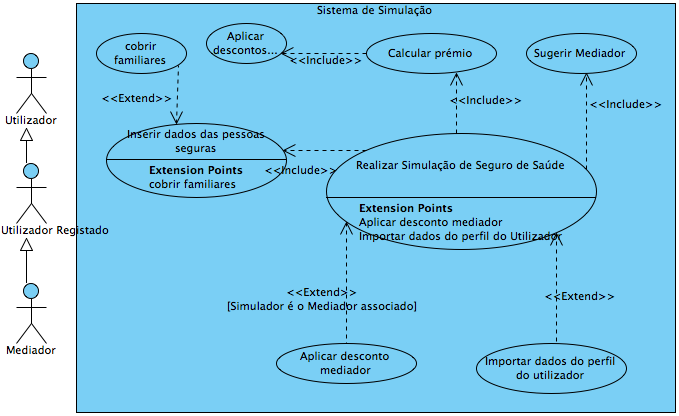
\includegraphics[scale=0.65]{images/Prints/RealizacaoSeguroSaude/SimulacaoSeguroSaude.png}
\end{figure}

\pagebreak

\subsection{Realizar Simulação de Seguro de Saúde}
\begin{figure}[!htb]
	\centering
	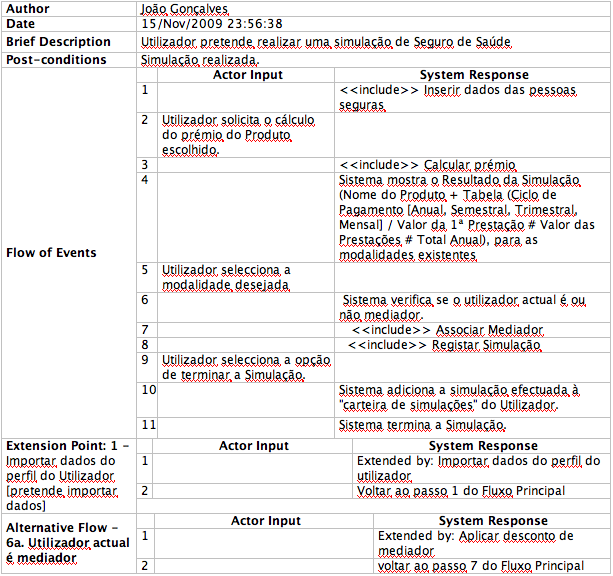
\includegraphics[scale=0.6]{images/Prints/RealizacaoSeguroSaude/RealizarSimulacaoSaude.png}
\end{figure}

\pagebreak

\subsection{Inserir dados das pessoas seguras}
\begin{figure}[!htb]
	\centering
	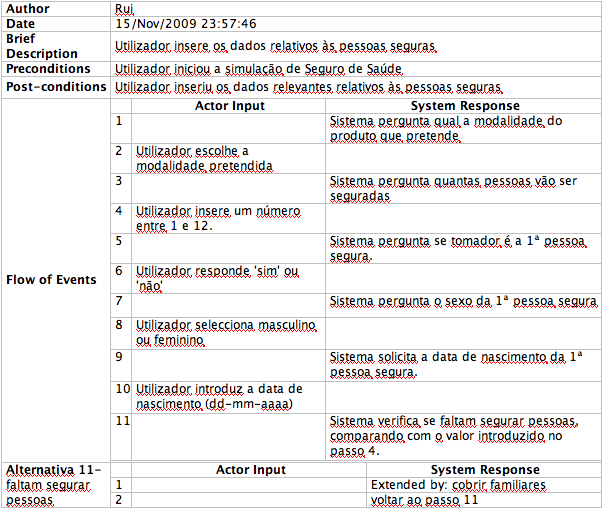
\includegraphics[scale=0.7]{images/Prints/RealizacaoSeguroSaude/InserirDadosPessoasSeguras.png}
\end{figure}

\pagebreak

\subsection{Cobrir Familiares}
\begin{figure}[!htb]
	\centering
	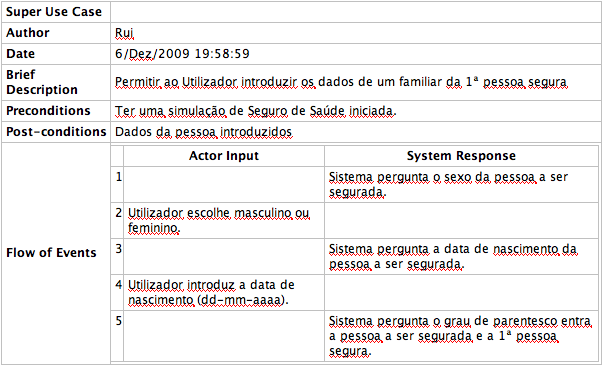
\includegraphics[scale=0.6]{images/Prints/RealizacaoSeguroSaude/CobrirFamiliares.png}
\end{figure}

\subsection{Cálculo do prémio da simulação saúde}
\begin{figure}[!htb]
	\centering
	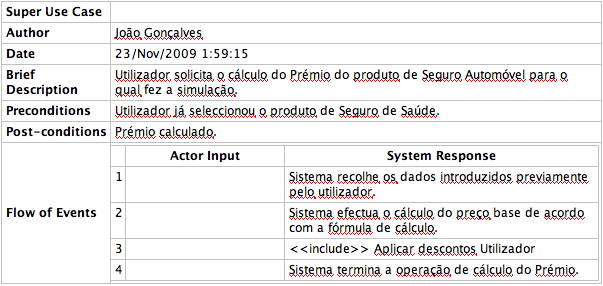
\includegraphics[scale=0.6]{images/Prints/RealizacaoSeguroSaude/CalcularPremio.png}
\end{figure}

\pagebreak

\subsection{Aplicação de descontos do utilizador}
\begin{figure}[!htb]
	\centering
	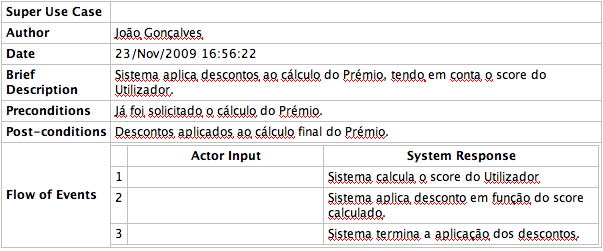
\includegraphics[scale=0.65]{images/Prints/RealizacaoSeguroSaude/AplicarDescontoUtilizador.png}
\end{figure}

\subsection{Aplicar o Desconto de Mediador}
\begin{figure}[!htb]
	\centering
	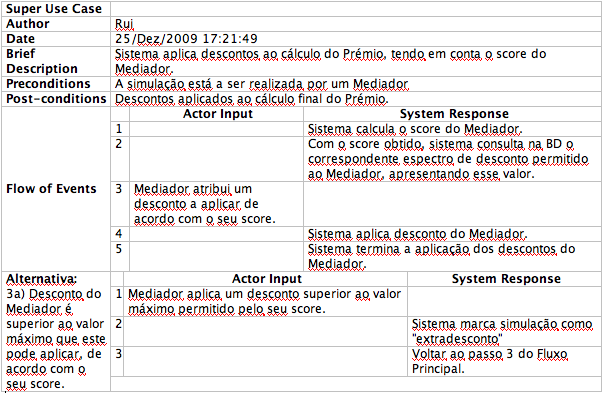
\includegraphics[scale=0.70]{images/Prints/RealizacaoSeguroSaude/AplicarDescontoMediador.png}
\end{figure}

\pagebreak

\subsection{Sugestão de mediador}
\begin{figure}[!htb]
	\centering
	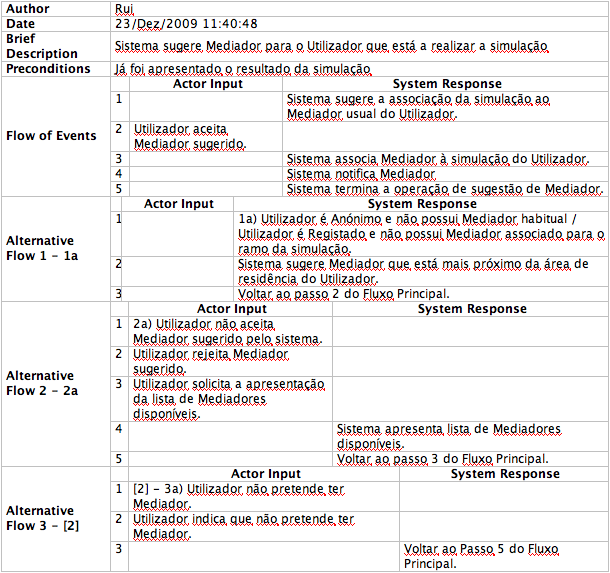
\includegraphics[scale=0.65]{images/Prints/RealizacaoSeguroSaude/SugerirMediador.png}
\end{figure}

\subsection{Importar dados do Utilizador}
\begin{figure}[!htb]
	\centering
	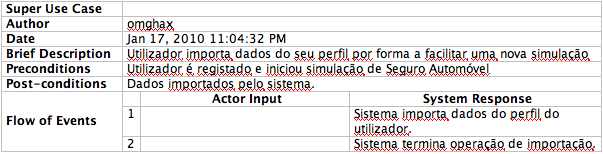
\includegraphics[scale=0.7]{images/Prints/RealizacaoSeguroSaude/ImportarDadosUtilizador.png}
\end{figure}

\pagebreak



\section{Contratação}
\begin{figure}[!htb]
	\centering
	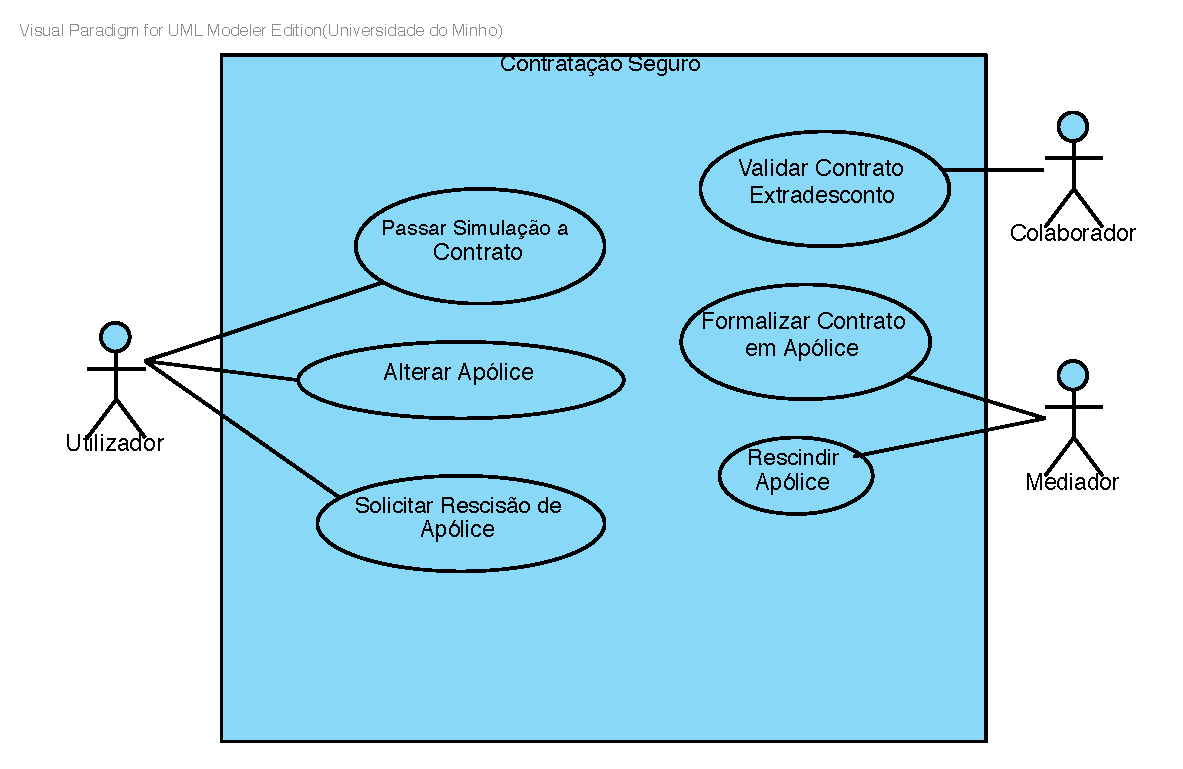
\includegraphics[scale=0.7]{images/Prints/Contratacao/Contratacao.pdf}
\end{figure}

\pagebreak

\subsection{Passar de simulação a contrato}
\begin{figure}[!htb]
	\centering
	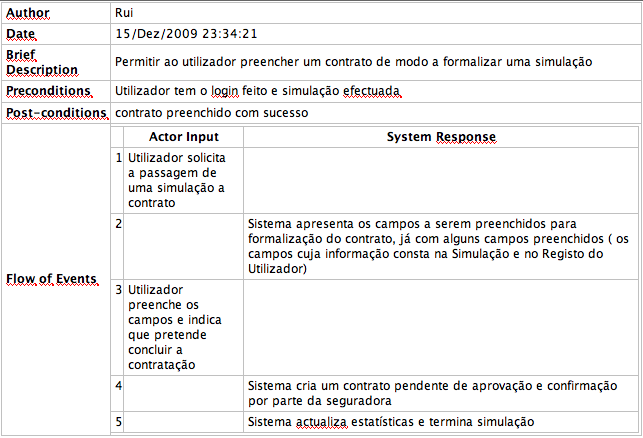
\includegraphics[scale=0.7]{images/Prints/Contratacao/PassarSimulacaoContrato.png} 
\end{figure}

\subsection{Solicitar Rescisão da Apólice}
\begin{figure}[!htb]
	\centering
	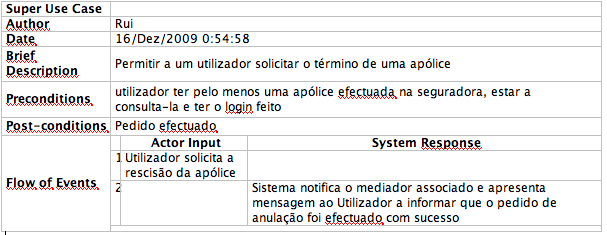
\includegraphics[scale=0.7]{images/Prints/Contratacao/SolicitarRescisaoApolice.png} 
\end{figure}


\pagebreak

\subsection{Alterar Apólice}
\begin{figure}[!htb]
	\centering
	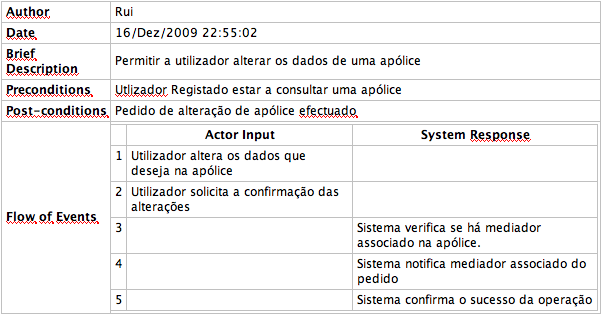
\includegraphics[scale=0.7]{images/Prints/Contratacao/AlterarApolice.png} 
\end{figure}

\subsection{Validar Extradesconto}
\begin{figure}[!htb]
	\centering
	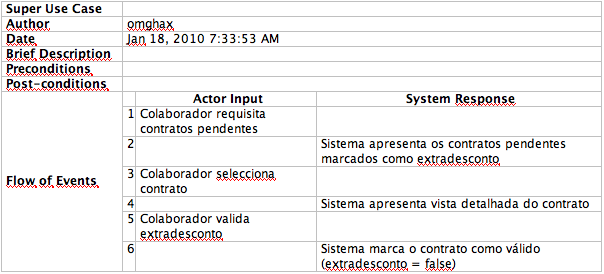
\includegraphics[scale=0.7]{images/Prints/Contratacao/ValidarContratoExtradesconto.png} 
\end{figure}

\pagebreak

\subsection{Formalizar Contrato em Apólice}
\begin{figure}[!htb]
	\centering
	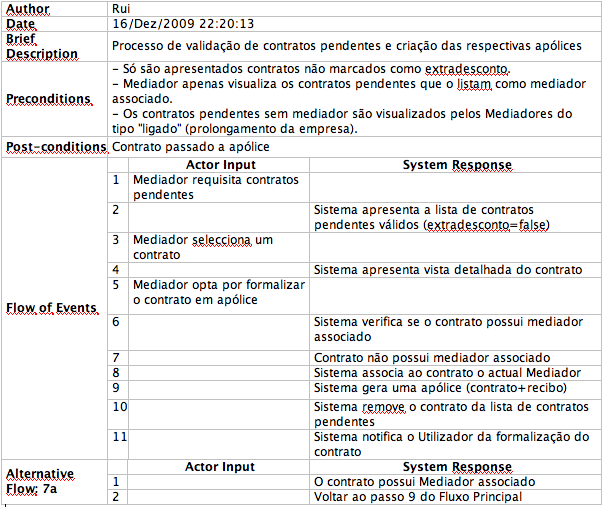
\includegraphics[scale=0.62]{images/Prints/Contratacao/FormalizarContratoApolice.png} 
\end{figure}

\subsection{Rescindir Apólice}
\begin{figure}[!htb]
	\centering
	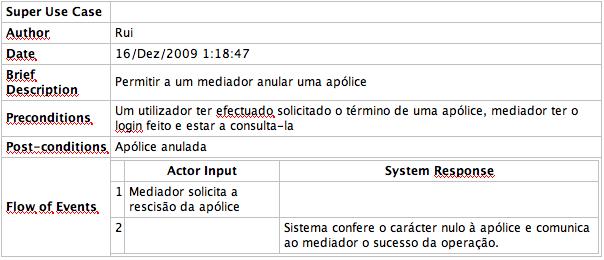
\includegraphics[scale=0.62]{images/Prints/Contratacao/RescindirApolice.png} 
\end{figure}

\pagebreak



\section{Configuração de Produtos}
\begin{figure}[!htb]
	\centering
	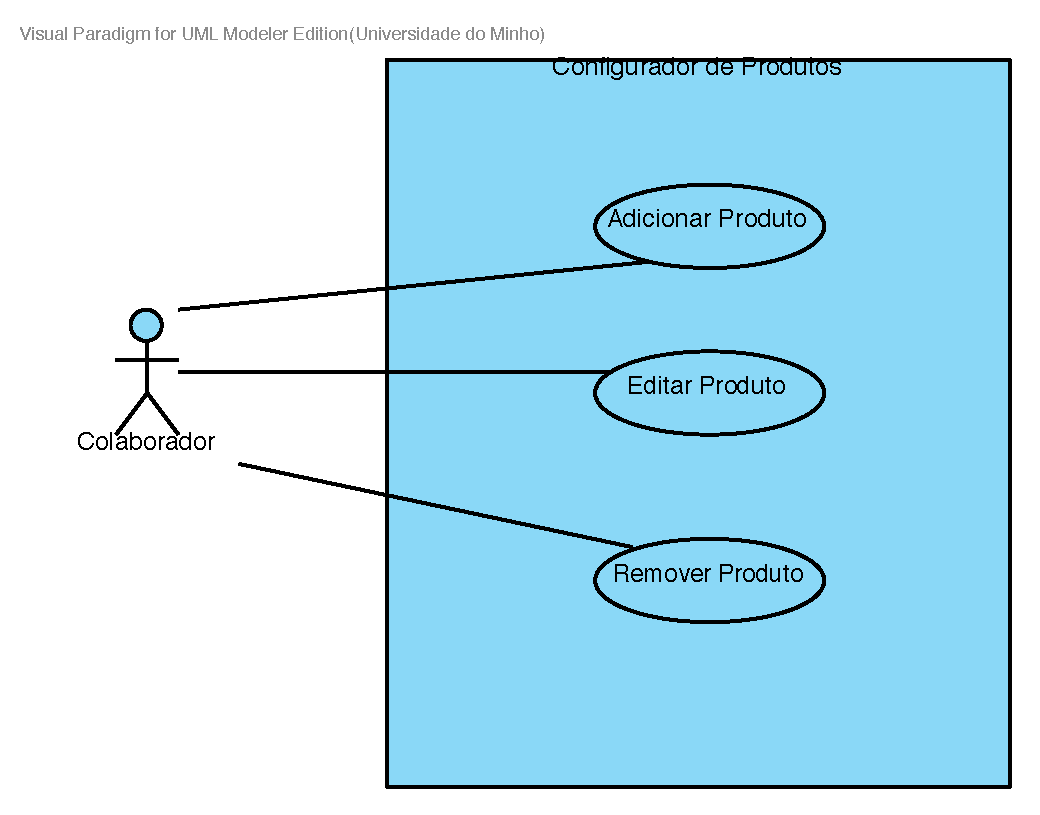
\includegraphics[scale=0.7]{images/Prints/ConfiguracaoProdutos/Produtos.pdf}
\end{figure}

\pagebreak

\subsection{Adicionar Produto}
\begin{figure}[!htb]
	\centering
	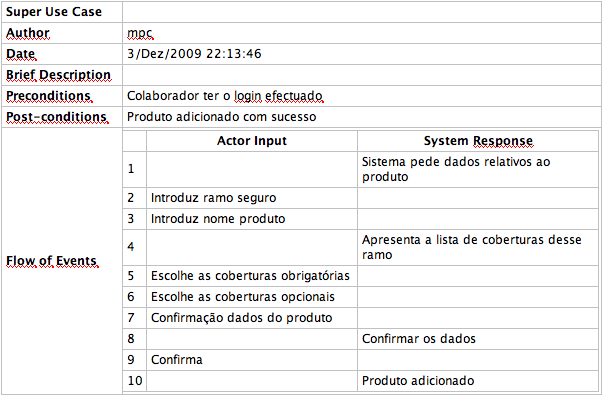
\includegraphics[scale=0.61]{images/Prints/ConfiguracaoProdutos/AdicionarProduto.png}
\end{figure}

\subsection{Remover Produto}
\begin{figure}[!htb]
	\centering
	\includegraphics[scale=0.50]{images/Prints/ConfiguracaoProdutos/RemoverProduto.png}
\end{figure}

\pagebreak

\subsection{Editar Produto}
\begin{figure}[!htb]
	\centering
	\includegraphics[scale=0.70]{images/Prints/ConfiguracaoProdutos/EditarProduto.png}
\end{figure}


\pagebreak


\section{Configuração de Descontos}
\begin{figure}[!htb]
	\centering
	\includegraphics[scale=0.7]{images/Prints/ConfiguracaoDescontos/ConfiguracaoDescontos.pdf}
\end{figure}

\pagebreak

\subsection{Adicionar Desconto}
\begin{figure}[!htb]
	\centering
	\includegraphics[scale=0.61]{images/Prints/ConfiguracaoDescontos/AdicionarDesconto.png}
\end{figure}

\pagebreak

\subsection{Remover Desconto}
\begin{figure}[!htb]
	\centering
	\includegraphics[scale=0.50]{images/Prints/ConfiguracaoDescontos/RemoverDesconto.png}
\end{figure}

\pagebreak

\subsection{Editar Descontos}
\begin{figure}[!htb]
	\centering
	\includegraphics[scale=0.60]{images/Prints/ConfiguracaoDescontos/EditarDesconto.png}
\end{figure}

\pagebreak



\section{Sugestão de Novas Simulacoes}
\begin{figure}[!htb]
	\centering
	\includegraphics[scale=0.6]{images/Prints/SugestaoNovasSimulacoes/SugestaoNovasSimulacoes.pdf}
\end{figure}

\subsection{Envio de sugestões}
\begin{figure}[!htb]
	\centering
	\includegraphics[scale=0.6]{images/Prints/SugestaoNovasSimulacoes/EnviarSugestao.png}
\end{figure}

\pagebreak


\section{Registo de Utilizadores}
\begin{figure}[!htb]
	\centering
	\includegraphics[scale=0.63]{images/Prints/RegistoUtilizadores/RegistoUtilizadores.pdf}
\end{figure}

\subsection{Login}
\begin{figure}[!htb]
	\centering
	\includegraphics[scale=0.63]{images/Prints/RegistoUtilizadores/Login.png}
\end{figure}

\pagebreak

\subsection{Registar}
\begin{figure}[!htb]
	\centering
	\includegraphics[scale=0.7]{images/Prints/RegistoUtilizadores/Registar.png}
\end{figure}

\pagebreak

\subsection{Recuperar Password}
\begin{figure}[!htb]
	\centering
	\includegraphics[scale=0.7]{images/Prints/RegistoUtilizadores/RecuperarPassword.png}
\end{figure}

\subsection{Criar Login}
\begin{figure}[!htb]
	\centering
	\includegraphics[scale=0.7]{images/Prints/RegistoUtilizadores/CriarLogin.png}
\end{figure}

\pagebreak

\subsection{Remover Login}
\begin{figure}[!htb]
	\centering
	\includegraphics[scale=0.7]{images/Prints/RegistoUtilizadores/RemoverLogin.png}
\end{figure}



%\chapter{Diagrama de Navegação}
%\section{Diagrama de Navegação}
%\begin{figure}
	\centering	
	\includegraphics[scale=0.8]{images/Prints/DiagramaNavegacao.pdf}
\end{figure}
\pagebreak
\end{document}
